
%\columnseprule=0.5pt 
%\columnsep=8pt

\begin{multicols}{2}    

\begin{enumerate}[leftmargin=20pt]

{\small
\subsection{函数}
\item 求$ y=\dfrac{Ax+B}{Cx+D}\ (AD-BC\neq 0) $的值域 
    \ifte \else (只需写出计算方法,无需具体结果) \fi:\\
\ifte  \underline{ {\scriptsize $
y= \dfrac{A}{C}\cdot\dfrac{x+
    \dfrac{D}{C}-\dfrac{D}{C}+ \dfrac{B}{A}}{x+\dfrac{D}{C}} \\
=\dfrac{A}{C}\cdot\left(
1+\dfrac{-\dfrac{D}{C}+\dfrac{B}{A}}{x+\dfrac{D}{C}}\right)$} }
 \else \\ \underline{\  \hspace{6cm}\ } \fi .

\item 设$ k>0,\ b>0 $,则$ y=kx+\dfrac{b}{x} $与
$ y=kx-\dfrac{b}{x} $的图像如下,这两种函数都是双曲线,
\begin{figure}[H]
    \centering
    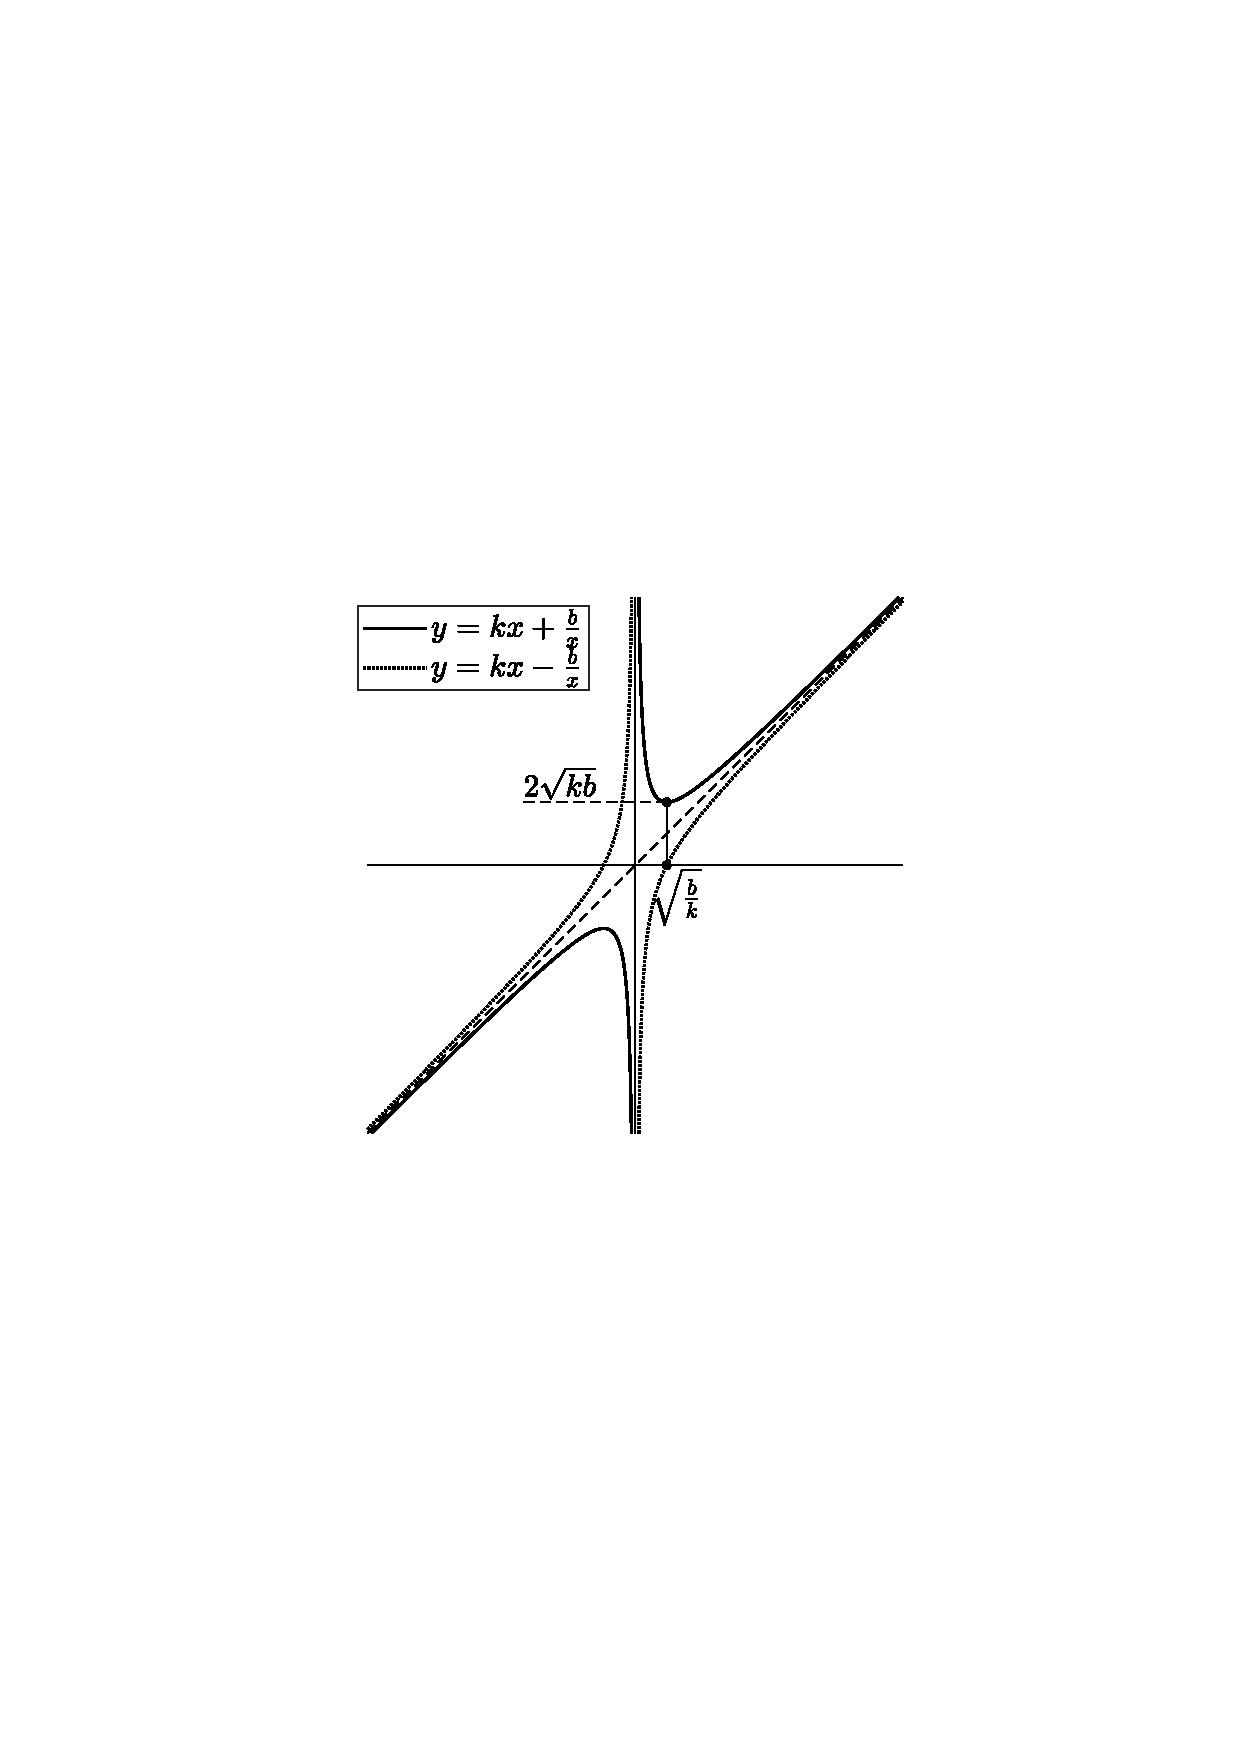
\includegraphics[width=0.5\linewidth]{两种双曲线_双钩与递增}
\end{figure}
当$ x>0 $时,
$ y=kx+\dfrac{b}{x} $在$ x=\underline{\ \ifte \sqrt{\dfrac{b}{k}}
  \else \hspace{1cm} \fi\ } $处取得极小值\underline{\ \ifte 
  $ 2\sqrt{kb} $\else \hspace{2cm} \fi\ };
$ y=kx-\dfrac{b}{x} $的零点是$ x=\underline{\ \ifte \sqrt{\dfrac{b}{k}}
    \else \hspace{1cm} \fi\ } $.

\item 求$ y=\dfrac{x^2+Ax+B}{x+C} $\ \ding{172}或
$ y=\dfrac{x+C}{x^2+Ax+B} $\ \ding{173}的值域
(若分子或分母的最高次项系数不为1,则先将系数提取出来),方法一:换元
\underline{\ \ifte $ t=x+C $\else \hspace{2cm} \fi\ };\\
方法二:\underline{\ \ifte 判别式\else \hspace{1.5cm} \fi\ },
以\ding{172}式为例写出主要过程:\ifte 
\begin{gather*}
    y(x+C)=x^2+Ax+B \\
    x^2+(A-y)x+B-yC=0 \\
    \Delta=(A-y)^2-4(B-yC) \geq 0
\end{gather*}
\else \vspace{1cm} \fi  

要绘制\ding{172}或\ding{173}的图像,
可以先绘制$ y=(x^2+Ax+B)(x+C) $的图像,
因为这个三次函数的正负号与\ding{172}或\ding{173}式的正负号是一致的。

\item 求$ y=\dfrac{\sqrt{Ax^2+B}}{Cx^2+D} $的值域,先提取系数,\\
$ y=\dfrac{\sqrt{A}}{C}\cdot\dfrac{\sqrt{x^2+\frac{B}{A}}}{
x^2+\frac{D}{C}} $,换元,$ t=\underline{\ \ifte 
\sqrt{x^2+\dfrac{B}{A}} \else \hspace{2cm} \fi\ } $,那么
$ x^2=t^2-\dfrac{B}{A} $,
\begin{gather*}
    y=\dfrac{\sqrt{A}}{C}\cdot \dfrac{t}{t^2-\dfrac{B}{A}+\dfrac{D}{C}}=
    \dfrac{\sqrt{A}}{C}\cdot \dfrac{1}{t+\left(\dfrac{D}{C}-\dfrac{B}{A}
    \right) \dfrac{1}{t}}
\end{gather*}

\item 给定4个实数$ x_1,x_2,x_3,x_4 $,其中任意两个都不相等,设
$ y_i=\dfrac{Ax_i+B}{Cx_i+D} $,$ (AD-BC\neq 0,\ i=1,2,3,4) $,那么,
\begin{gather*}
    \dfrac{(y_1-y_3)(y_2-y_4)}{(y_1-y_4)(y_2-y_3)}=
    \dfrac{(x_1-x_3)(x_2-x_4)}{(x_1-x_4)(x_2-x_3)}
\end{gather*}

\item $ y=|x-b_1|+|x-b_2|+\cdots+|x-b_n| $,假设$ b_1<b_2<\cdots<b_n $,
如果$ n $是偶数,那么最小值在区间
\underline{\ \ifte $ [b_{\frac{n}{2}},
b_{\frac{n}{2}+1}] $\else \hspace{2cm} \fi\ }
内取得;如果$ n $是奇数,那么最小值在\underline{\ 
\ifte $ x=b_{\frac{n+1}{2}} $\else \hspace{2cm} \fi\ }处取得。

\item 恒成立问题或有解问题($ \exists $表示存在,$ \forall $表示任意。
$ f(x)_{\max},f(x)_{\min} $分别表示$ f(x) $在区间$ (a,b) $上的最大值、最小值。)
\begin{align*}
    \exists\ x_0\in(a,b),\ f(x_0)>m &\ \Rightarrow \ 
    \underline{\ \ifte f(x)_{\max} >m\else \hspace{2cm} \fi\ }\\
    \exists\ x_0\in(a,b),\ f(x_0)<m &\ \Rightarrow \ 
    \underline{\ \ifte f(x)_{\min} <m\else \hspace{2cm} \fi\ }\\
    \forall\ x\in(a,b),\ f(x)<m &\ \Rightarrow \ 
    \underline{\ \ifte f(x)_{\max} <m\else \hspace{2cm} \fi\ }\\
    \forall\ x\in(a,b),\ f(x)>m &\ \Rightarrow \ 
    \underline{\ \ifte f(x)_{\min} >m\else \hspace{2cm} \fi\ }
\end{align*}

\item 对数运算法则:\\ $ \log_a (MN)= $\underline{\ \ifte 
    $ \log_a M+\log_a N $ \else \hspace{2cm} \fi\ }. \\
$ \log_a \Big(\dfrac{M}{N}\Big)= $\underline{\ \ifte 
    $ \log_a M-\log_a N $ \else \hspace{2cm} \fi\ }. \\
$ \log_a M^n= $\underline{\ \ifte 
    $ n\log_a M $ \else \hspace{1.5cm} \fi\ },\q 
$ \log_{a^n} M= $\underline{\ \ifte 
    $ \dfrac{1}{n}\log_a M $ \else \hspace{1.5cm} \fi\ }. \\
换底公式:$ \log_a M= $\underline{\ \ifte 
    $ \dfrac{\log_b M}{\log_b a} $ \else \hspace{2cm} \fi\ }.

\item 写出符合以下函数方程的函数:
{\footnotesize \begin{align*}
&f(x_1+x_2)=f(x_1)+f(x_2)   	
    &\underline{\ \ifte kx\else \hspace{0.7cm} \fi\ } \\
&f\left(\dfrac{x_1+x_2}{2}\right) =\dfrac{f(x_1)+f(x_2)}{2}  
    &\underline{\ \ifte kx+b\else \hspace{0.7cm} \fi\ }\\
&f(x_1x_2)=f(x_1)f(x_2)   	
    & \underline{\ \ifte x^{\alpha}\else \hspace{0.7cm} \fi\ }\\
&f(x_1+x_2)=f(x_1)f(x_2)   	
    &\underline{\ \ifte a^x\else \hspace{0.7cm} \fi\ }\\
&f(x_1x_2)=f(x_1)+f(x_2)   	
    &\underline{\ \ifte \log_{a}x\else \hspace{0.7cm} \fi\ } \\
&f(x_1x_2)=x_2f(x_1)+x_1f(x_2)   	
    &\underline{\ \ifte x\log_{a}x\else \hspace{0.7cm} \fi\ } \\
& f(x_1+x_2)+f(x_1-x_2)=2\lambda f(x_1)f(x_2)
    &\underline{\ \ifte \dfrac{1}{\lambda}\cos x \else \hspace{0.7cm} \fi\ } \\
& f(x_1+x_2)= f(x_1)+f(x_2)+2\lambda x_1x_2
    &\underline{\ \ifte \lambda x^2+\mu x \else \hspace{0.7cm} \fi\ } 
\end{align*} }

\item $^*$ $ f(x)=\ln \dfrac{1+x}{1-x} $或$ f(x)=\ln \dfrac{1-x}{1+x} $,则
\begin{gather*}
    f(x_1)+f(x_2)=f\left(\underline{\ \ifte \dfrac{x_1+x_2}{1+x_1x_2}
        \else \hspace{1cm} \fi\ } \right)
\end{gather*}

\item $ \arctan x_1+\arctan x_2=\underline{\ \ifte 
  \arctan\dfrac{x_1+x_2}{1-x_1x_2} \else \hspace{2cm} \fi\ } $.

\item 函数凹凸性,填“$ < $”或“$ > $”,请结合图像记忆。\\
$ x_1,x_2\in (0,\pi),\ x_1\neq x_2 $,
\begin{align*}
    \dfrac{1}{2} \left(\sin x_1 + \sin x_2 \right) 
    \underline{\ \ifte < \else \hspace{1cm} \fi\ }
    \sin \dfrac{x_1+x_2}{2}
\end{align*}
$ x_1,x_2\in (0,\dfrac{\pi}{2}),\ x_1\neq x_2 $,
\begin{align*}
    \dfrac{1}{2}\left(\tan x_1+\tan x_2\right)
    \underline{\ \ifte > \else \hspace{1cm} \fi\ }
    \tan\dfrac{x_1+x_2}{2}
\end{align*}
$ x_1,x_2\in \textbf{R},\ x_1\neq x_2 $,
\begin{align*}
    \dfrac{\e^{x_1}+\e^{x_2}}{2}
    \underline{\ \ifte > \else \hspace{1cm} \fi\ }
    \e^{\frac{x_1+x_2}{2}}
\end{align*}
$ x_1,x_2\in (0,+\infty),\ x_1\neq x_2 $,
\begin{align*}
    \dfrac{\ln x_1+\ln x_2}{2}
    \underline{\ \ifte < \else \hspace{1cm} \fi\ }
    \ln\dfrac{x_1+x_2}{2}
\end{align*}
$ x_1,x_2\in (0,+\infty),\ x_1\neq x_2,
\ \alpha\in \textbf{R},\ \alpha>1 $,
\begin{gather*}
    \dfrac{x_1^{\alpha}+x_2^{\alpha}}{2}
    \underline{\ \ifte > \else \hspace{1cm} \fi\ }
    \left( \dfrac{x_1+x_2}{2}\right)^{\alpha}
\end{gather*}

\item 若$ f(x) $满足$ f(x)=\pm\dfrac{1}{f(x+a)} $,那么
$ f(x) $的一个周期是\underline{\ \ifte $ 2a $ \else \hspace{1cm} \fi\ }.

\item 若$ f(x) $满足$ f(x+a)=f(b-x) $,则$ f(x) $的一条对称轴是
\underline{\ \ifte $ x=\dfrac{a+b}{2} $ \else \hspace{2cm} \fi\ }.  

\item 如果$ f(x) $同时具有对称轴$ x=a $和对称中心$ (b,c) $,且$ a\neq b $,
那么$ f(x) $具有周期$ T=\underline{\ \ifte 4|a-b|\else \hspace{1cm} \fi\ } $.

\item 三变量均值不等式:设$ a,b,c\geq 0 $,则$ \dfrac{a+b+c}{3}\geq 
\underline{\ \ifte \sqrt[3]{abc}\else \hspace{1cm} \fi\ } $.

\item 设$ a,b>0,x>0 $,利用上面的三变量均值不等式,有:\\
$ ax^2+\dfrac{b}{x}=ax^2+\dfrac{b}{2x}+\dfrac{b}{2x}\geq 
\underline{\ \ifte 3 \sqrt[3]{\dfrac{ab^2}{4}}\else \hspace{2cm} \fi\ } $;\\
$ ax+\dfrac{b}{x^2}=\dfrac{1}{2}ax+\dfrac{1}{2}ax+\dfrac{b}{x^2} \geq 
\underline{\ \ifte 3 \sqrt[3]{\dfrac{a^2b}{4}}\else \hspace{2cm} \fi\ } $.

\item 零点存在定理:若函数$ f(x) $在闭区间$ [a,b] $连续,
且$ f(a)\cdot f(b)\underline{\ \ifte <0\else \hspace{1cm} \fi\ } $,
则一定存在$ x_0\in(a,b) $,使$ f(x_0)=0 $.
此定理为二分法找函数零点的理论基础。

\item $^*$ 记$ f_0(x)=x,\ f_1(x)=f(x),\ f_{n+1}(x)=f(f_n(x)) $. 
称$ f_n(x) $为函数$ f(x) $的$ n $次迭代 \ifte 
(用数学归纳法证明) \fi。
\renewcommand\arraystretch{1.5} 
%\vspace{1mm} 
\\  
\begin{tabular}{|c|c|} 
    \hline
    $ f(x) $ & $ f_n(x) $ \\
    \hline
    $ x+2\sqrt{x}+1 $ & \ifte $ (\sqrt{x}+n)^2 $\else \hspace{3cm}  \fi \\
    \hline
    $ \dfrac{x}{a+bx} $ & \ifte $ \dfrac{x}{a^n+\dfrac{1-a^n}{1-a}bx} $ \fi \\
    \hline
    $ \sqrt[k]{ax^k+b} $ & \ifte $ \sqrt[k]{a^nx^k+\dfrac{1-a^n}{1-a}b} $ \fi \\
    \hline
    $ x^2+2x $ & \ifte $ (x+1)^{2^n}-1 $ \fi \\
    \hline
    $ \dfrac{x^2}{2x-1} $ & $\dfrac{x^{2^n}}{x^{2^n}-(x-1)^{2^n}}$ \\
    \hline
\end{tabular} \\

\item $\ f_1(x)=f(x)=\dfrac{1+x}{1-x},\ f_{n+1}(x)=f(f_n(x)) $,
$ n\in \textbf{N}^+ $,$ k\in \textbf{N} $,
则\\ $ f_{4k+1}(x)=\underline{\ \ifte 
\dfrac{1+x}{1-x} \else \hspace{1cm} \fi\ } $,
$ f_{4k+2}(x)=\underline{\ \ifte -\dfrac{1}{x}
\else \hspace{1cm} \fi\ } $, \\ $ f_{4k+3}(x)=\underline{\ \ifte 
\dfrac{x-1}{x+1} \else \hspace{1cm} \fi\ } $,
$ f_{4k+4}(x)=\underline{\ \ifte x\else \hspace{1cm} \fi\ } $.


\subsection{排列、组合与二项式定理}
\item 排列数:$ P_n^k= $\underline{\ \ifte $ \dfrac{n!}{(n-k)!} $
     \else \hspace{2cm} \fi\ },或者写成$ A_n^k $. 

\item 组合数:$ C_n^k=C_n^{n-k}= $\underline{\ \ifte 
$ \dfrac{n!}{k!(n-k)!} $ \else \hspace{2cm} \fi\ }. \\
递推关系:$ C_n^k+C_n^{k-1}= $\underline{\ \ifte $ C_{n+1}^k $ 
\else \hspace{2cm} \fi\ }. 

\item 二项式定理:$ (a+b)^n= $ \underline{\ \ifte 
$ \sum\limits_{k=0}^nC_n^ka^kb^{n-k} $ \else \hspace{2cm} \fi\ }.

\item $ (a+b+c)^2 = $\underline{\ \ifte 
    $ a^2+b^2+c^2+2(ab+ac+bc) $ \else \hspace{4.5cm} \fi\ }. \\
$ (\vec{a}+\vec{b}+\vec{c})^2 $的结果类似。

\item 杨辉三角:
\vspace{-3mm}
\begin{gather*}
    1 \\
    1\q 1 \\
    1\q 2 \q 1 \\
    \ifte 
    \underline{1\q 3 \q 3 \q 1} \\
    \underline{1\q 4 \q 6 \q 4 \q 1} \\
    \underline{1\q 5 \q 10 \q 10 \q 5 \q 1} \\
    \underline{1\q 6 \q 15 \q 20 \q 15 \q 6 \q 1} 
    \else
    \underline{\hspace{2cm}} \\
    \underline{\hspace{3cm}} \\
    \underline{\hspace{4cm}} \\
    \underline{\hspace{5cm}}   
    \fi 
\end{gather*}
第$ n+1 $行的系数之和为$ \sum\limits_{k=0}^{n} C_n^k=
\underline{\ \ifte 2^{n} \else \hspace{2cm} \fi\ } $.

\item $^*$ $ C_{2n}^1 $,$ C_{2n}^3 $,$ C_{2n}^5,\cdots,C_{2n}^{2m-1}\ (1\leq m\leq n) $
都是\underline{\ \ifte 偶\else \hspace{0.5 cm} \fi\ }数。
(填“奇”或“偶”)

\item $^*$ 组合恒等式:
\begin{align*}
&\sum_{k=r}^{n} C_k^r=\underline{\ \ifte C_{n+1}^{r+1}
     \else \hspace{2cm} \fi\ } \\
&\sum_{k=0}^{r}C_m^kC_n^{r-k}=\underline{\ \ifte 
    C_{n+m}^r \else \hspace{2cm} \fi\ }  \\
&\sum_{k=1}^{n} kC_n^k=\underline{\ \ifte n\cdot2^{n-1} 
     \else \hspace{2cm} \fi\ } \\ 
&\sum_{k=1}^{n} k^2C_n^k=\underline{\ \ifte 
    n(n+1)\cdot2^{n-2} \else \hspace{2cm} \fi\ } 
\end{align*}

\item $^*$ 设$ n $个元素错排的方案数为$ D_n $,$ D_1=0,\ D_2=1 $,则
\begin{gather*}
    D_n =(n-1)(D_{n-1}+D_{n-2}) \\
    D_n-nD_{n-1}=-[D_{n-1}-(n-1)D_{n-2}]=(-1)^n \\
    \dfrac{D_n}{n!}-\dfrac{D_{n-1}}{(n-1)!}=\dfrac{(-1)^n}{n!} \\
    D_n= n!\left[ 1-\dfrac{1}{1!}+\dfrac{1}{2!}-\cdots 
    +(-1)^n\dfrac{1}{n!}\right]
\end{gather*}

\item $ \left(ax^{\alpha}+bx^{\beta} \right)^n $展开式的通项为
\begin{gather*}
    T_{r+1}=C_n^ra^{n-r}b^rx^{(n-r)\alpha+r\beta} ,
\end{gather*}
设$ C_n^m a^{n-m}b^m $是最大的系数,则
\begin{align*}
\begin{dcases}
    C_n^m a^{n-m}b^m\geq \underline{\ \ifte 
      C_n^{m-1} a^{n-m+1}b^{m-1} \else \hspace{3cm} \fi\ } \\
    C_n^m a^{n-m}b^m\geq \underline{\ \ifte 
      C_n^{m+1} a^{n-m-1}b^{m+1}\else \hspace{3cm} \fi\ }
\end{dcases}
\end{align*} 

\item 设$ k\in \mathbf{N} $,在$ 30k+1 $到$ 30k+30 $
这连续30个整数中,不是2或3或5的倍数的整数一共有
\underline{\ \ifte 8 \else \hspace{0.5 cm} \fi\ } 个
\ifte (恰好是一个字节包含的bit数) \else \fi。

\subsection{概率论与数理统计}

\item 给定正整数集合$ S=\{k_1,k_2,\cdots,k_n\} $,定义多项式
$ f(x)=(1+x^{k_1})(1+x^{k_2})\cdots (1+x^{k_n}) $,则
$ f(x) $的展开式中,\underline{\ \ifte $ x^m $的系数\else 
\hspace{2cm} \fi\ }恰好等于从集合$ S $中选出元素总和为
$ m\ (m\in \textbf{N}) $的子集的方法数。

\item 数学期望(或均值)的定义:$ E(X)=\underline{\ \ifte 
\sum\limits_{i=1}^{n}x_ip_i \else \hspace{2cm} \fi\ } $,\\ 
性质:$ E(aX+b)=\underline{\ \ifte
aE(X)+b \else \hspace{2cm} \fi\ } $. \\
方差:$ D(X)=E\{[X-E(X)]^2\}=\\ \underline{\ \ifte E(X^2)-[E(X)]^2
\else \hspace{2cm} \fi\ } $,\\ 性质:$ D(aX+b)=\underline{\ \ifte
a^2D(X) \else \hspace{2cm} \fi\ } $. 

\item 伯努利大数定律:独立地重复一个伯努利试验$ n $次,当$ n $很大时,
频率逼近\underline{概率}。

\item 概率加法公式:
\begin{gather*}
    P(A_1\cup A_2)=\underline{\ \ifte 
    P(A_1)+P(A_2)-P(A_1\cap A_2) \else \hspace{4cm} \fi\ }
\end{gather*}

\item 条件概率公式:$ P(B\mid A)=\underline{\ \ifte 
\dfrac{P(A\cap B)}{P(A)}\else \hspace{2cm} \fi\ } $. \\
概率乘法公式:$  P(A\cap B)=\underline{\ \ifte 
    P(A)P(B|A) \else \hspace{2cm} \fi\ } $. \\
若$ A,B $相互独立,则$ P(A\cap B)=\underline{\ \ifte 
    P(A)P(B) \else \hspace{2cm} \fi\ } $.

\item 全概率公式:$ P(A)=\underline{\ \ifte 
\sum\limits_{k=1}^{n} P(A \mid \varOmega_{k}) P(\varOmega_{k})
\else \hspace{3cm} \fi\ } $.

\item $^*$ 贝叶斯公式:
\begin{gather*}
    P(\varOmega_{i} \mid A)=\underline{\ \ifte 
    \dfrac{P(A \mid \varOmega_{i}) 
    P(\varOmega_{i})}{\sum\limits_{k=1}^{n} P(A \mid 
    \varOmega_{k}) P(\varOmega_{k})} \else \hspace{3cm} \fi\ }
\end{gather*}

\item 二项分布$ b(n,p) $:每次实验时,事件$ A $发生的概率为
$ p $,那么在$ n $次实验中事件$ A $发生$ k $次的概率为
$ P\{X=k\}= $\underline{\ \ifte $ C_n^kp^k(1-p)^{n-k} $
    \else \hspace{2cm} \fi\ }. 数学期望为\underline{\ \ifte 
$ np $ \else \hspace{1cm} \fi\ },方差为\underline{\ \ifte 
$ np(1-p) $ \else \hspace{2cm} \fi\ }. 

\item $^*$ 几何分布:在$ n $次伯努利试验中,试验$ k $次才得到第一次成功的概率,$ P\{X=k\}=(1-p)^{k-1}p ,\ k\in \textbf{N}^+,\ 0<p<1 $. 
数学期望为\underline{\ \ifte $ \dfrac{1}{p} $\else \hspace{1cm} \fi\ },
方差为\underline{\ \ifte $ \dfrac{1-p}{p^2} $\else \hspace{2cm} \fi\ }. 

\item 超几何分布:共有$ N $件产品,其中有$ D (D\leq N) $件次品,
从中任取$ n(n\leq N)$件,其中恰有$ k(k\leq D) $件次品的概率:
$ P\{X=k\}=\underline{\ \ifte \dfrac{C_D^kC_{N-D}^{n-k}}{C_N^n}
\else \hspace{2cm} \fi\ } $. 数学期望为\underline{\ \ifte 
$ \dfrac{nD}{N} $\else \hspace{1cm} \fi\ },
方差为$ \dfrac{nD}{N}\Big(1-\dfrac{D}{N}
\Big)\Big(\dfrac{N-n}{N-1}\Big) $.

\item 正态分布:$ f(x)=\dfrac{1}{\sqrt{2\pi}\sigma}\e^{-\frac{(x-\mu)^2}
    {2\sigma^2}},\ \mu \in \textbf{R},\ \sigma>0 $. 数学期望为
\underline{\ \ifte $ \mu $\else \hspace{1cm} \fi\ },方差为
\underline{\ \ifte $ \sigma^2 $\else \hspace{1cm} \fi\ }. 
若$ X\sim N(\mu,\sigma^2) $,则$ \dfrac{X-\mu}{\sigma}
\sim \underline{\ \ifte N(0,1)\else \hspace{1.5cm} \fi\ } $
\ (标准正态分布). 

\item 最小二乘法,回归直线$ \hat{y}=\hat{a}+\hat{b}x $. 
\begin{align*}
    \hat{b} &=\dfrac{\sum\limits_{i=1}^{n}(x_i-\overline{x})(y_i-\overline{y})}{
        \sum\limits_{i=1}^{n}(x_i-\overline{x})^2}     
    =\dfrac{\sum\limits_{i=1}^{n}x_iy_i-n\overline{x}\, \overline{y}}{\sum\limits_{i=1}^{n}x_i^2-n\overline{x}^2} \\
    &=\dfrac{n\sum\limits_{i=1}^{n}x_iy_i-
        \Big(\sum\limits_{i=1}^{n}x_i\Big)
        \Big(\sum\limits_{i=1}^{n}y_i\Big)}{n\sum\limits_{i=1}^{n}x_i^2-
        \Big(\sum\limits_{i=1}^{n}x_i\Big)^2}\\
    \hat{a} &=\overline{y}-\hat{b}\overline{x}
\end{align*}
回归直线通过散点图的几何中心$ (\overline{x},\overline{y}) $. 

\item 样本相关系数
\begin{align*}    
    r &=\dfrac{\sum\limits_{i=1}^{n}(x_i-\overline{x})(y_i-\overline{y})}
    { \sqrt{\sum\limits_{i=1}^{n}(x_i-\overline{x})^2}\cdot 
        \sqrt{\sum\limits_{i=1}^{n}(y_i-\overline{y})^2} } \\
    &=\dfrac{\sum\limits_{i=1}^{n}x_iy_i-n\overline{x}\, \overline{y}}
    {\sqrt{\sum\limits_{i=1}^{n}x_i^2-n\overline{x}^2}\cdot 
     \sqrt{\sum\limits_{i=1}^{n}y_i^2-n\overline{y}^2}} \\
    &=\dfrac{n\sum\limits_{i=1}^{n}x_iy_i-\Big(\sum\limits_{i=1}^{n}x_i\Big)
        \Big(\sum\limits_{i=1}^{n}y_i\Big)}{
        \sqrt{n\sum\limits_{i=1}^{n}x_i^2-\Big(\sum\limits_{i=1}^{n}x_i\Big)^2}\cdot
        \sqrt{n\sum\limits_{i=1}^{n}y_i^2-\Big(\sum\limits_{i=1}^{n}y_i\Big)^2} } 
\end{align*}

\item (卡方)独立性检验,$ 2\times 2 $列联表:
\begin{table}[H]
    \centering
    \begin{tabular}{|c|c|c|c|}
        \hline
        & $ Y=0 $ & $ Y=1 $ & 合计 \\ \hline
        $ X=0 $ & $ a $ & $ b $ & $ a+b $ \\ \hline
        $ X=1 $ & $ c $ & $ d $ & $ c+d $ \\ \hline
        合计    & $ a+c $ & $ b+d $ & $ n=a+b+c+d $ \\ \hline
    \end{tabular}
\end{table}
\vspace{-8mm} 
\begin{align*}
    \chi^2 =\dfrac{n(ad-bc)^2}{(a+b)(c+d)(a+c)(b+d)}
\end{align*} 
$ \chi^2 $越大,说明“$ X $与$ Y $有关系”成立的可能性越大。

\subsection{三角函数}
\item 正余弦和角、差角公式:
\begin{align*} 
    \cos(\alpha\pm\beta )=&\ \underline{\ \ifte 
    \cos\alpha\cos\beta \mp \sin\alpha\sin\beta 
    \else \hspace{5cm} \fi\ } \\
    \sin(\alpha\pm\beta )=&\ \underline{\ \ifte 
    \sin\alpha\cos\beta \pm \cos\alpha\sin\beta    
        \else \hspace{5cm} \fi\ } 
\end{align*}

\item 二倍角公式:
{\footnotesize \begin{align*}
    & \sin 2x=\underline{\ \ifte 2\sin x\cos x
        \else \hspace{3cm} \fi\ } \\    
    & \cos 2x=\underline{\ \ifte  2\cos^2 x-1=1-2
     \sin^2 x=\cos^2 x- \sin^2 x\else \hspace{5cm} \fi\ }
\end{align*} }
\ifte \else (余弦二倍角需写出三种形式) \fi

\item $^*$ 三倍角公式:
\begin{align*} 
    & \sin 3x=\underline{\ \ifte -4 \sin^3 x+ 3\sin x
        \else \hspace{3cm} \fi\ } 	  \\	
    & \cos 3x=\underline{\ \ifte 4 \cos^3 x- 3\cos x
        \else \hspace{3cm} \fi\ } 
\end{align*}


\item 余弦的递推关系:
\begin{gather*}
    \cos(n+1)\theta=2\cos\theta\cos n\theta-\underline{\ 
        \ifte \cos(n-1)\theta \else \hspace{2cm} \fi\ } 
\end{gather*}

\item 和差化积:
\begin{align*}
    \sin x+\sin y=&\ \underline{\ \ifte 2\sin \left(\dfrac{x+y}{2}
    \right) \cos\left(\dfrac{x-y}{2}\right)\else \hspace{5cm} \fi\ } \\ 
    \cos x+\cos y=&\ \underline{\ \ifte 2\cos \left(\dfrac{x+y}{2}\right) \cos  \left(\dfrac{x-y}{2}\right) \else \hspace{5cm} \fi\ }
\end{align*}

\item 积化和差:
\begin{align*}
    \sin x\sin y=&\ \underline{\ \ifte 
        \dfrac{1}{2}[\cos(x-y)-\cos(x+y)]
        \else \hspace{5cm} \fi\ } \\
    \cos x\cos y=&\ \underline{\ \ifte 
        \dfrac{1}{2}[\cos(x-y)+\cos(x+y)]
        \else \hspace{5cm} \fi\ } \\	
    \sin x\cos y=&\ \underline{\ \ifte 
        \dfrac{1}{2}[\sin(x+y)+\sin(x-y)] 
        \else \hspace{5cm} \fi\ }
\end{align*}

\item 辅助角公式:
\begin{align*}
     &\ a\sin x+b\cos x\\
    =&\ \underline{\ \ifte 
        \sqrt{a^2+b^2}\sin(x+\varphi)
        \else \hspace{4cm} \fi\ } \qquad
    \left(\tan \varphi=\dfrac{b}{a}\right)
\end{align*}
变体一:
\begin{align*}
     &\ a\sin x+b\cos (x+x_0) \\
    =&\ \underline{\ \ifte 
        a\sin x+b\cos x\cos x_0-b\sin x\sin x_0
        \else \hspace{5cm} \fi\ } 
\end{align*}
变体二:
\begin{align*}
     &\ a\cos^2x+b\sin^2x+c\sin x\cos x \\
    =&\ \underline{\ \ifte
    a\dfrac{\cos2x+1}{2} +b\dfrac{-\cos2x+1}{2}+
    \dfrac{c}{2}\sin2x  \else \hspace{5cm} \fi\ } 
\end{align*}
变体三:
\begin{align*}
    a\sin^2x+b\cos x=\underline{\ \ifte 
        a(1-\cos^2x)+b\cos x
        \else \hspace{4cm} \fi\ }
\end{align*}

\item $^*$ 
\begin{align*}
    &\sum_{k=1}^{n}\cos kx=\underline{\ \ifte 
    \dfrac{\sin\left( n+\dfrac{1}{2}\right) x-\sin 
        \dfrac{x}{2}}{2\sin \dfrac{x}{2}}    
        \else \hspace{4.5cm} \fi\ }  \\
    &\sum_{k=1}^{n}\sin kx=\underline{\ \ifte 
        \dfrac{-\cos\left( n+\dfrac{1}{2}\right) x+\cos 
        \dfrac{x}{2}}{2\sin \dfrac{x}{2}}
        \else \hspace{4.5cm} \fi\ }
\end{align*}

\item $^*$ $ \cos\dfrac{x}{2} \cos\dfrac{x}{4}\cdots\cos\dfrac{x}{2^n}
=\underline{\ \ifte \dfrac{\sin x}{2^n \sin\dfrac{x}{2^n}}
    \else \hspace{2cm} \fi\ } $.

\item $^*$ $ \Delta ABC $中的恒等式($ A+B+C=\pi $):
\begin{align*} 
    &\sin A +\sin B +\sin C =\underline{\ \ifte 
        4\cos\left(\tfrac{A}{2}\right)\cos\left(\tfrac{B}{2}\right)
        \cos\left(\tfrac{C}{2}\right)\else \hspace{3cm} \fi\ }  \\
    &\cos A +\cos B +\cos C =\underline{\ \ifte 
        1+4\sin\left(\tfrac{A}{2}\right)\sin\left(\tfrac{B}{2}\right)
        \sin\left(\tfrac{C}{2}\right)\else \hspace{3cm} \fi\ }  \\
    &\tan A+\tan B +\tan C =\underline{\ \ifte 
        \tan A \tan B\tan C \else \hspace{3cm} \fi\ } \\
    &\tan\left(\tfrac{A}{2}\right)\tan\left(\tfrac{B}{2}\right)+
    \tan\left(\tfrac{B}{2}\right)\tan\left(\tfrac{C}{2}\right)+\\
    &\tan\left(\tfrac{A}{2}\right)\tan\left(\tfrac{C}{2}\right)=
    \underline{\ \ifte 1\else \hspace{1cm} \fi\ } 
\end{align*}

\item 对于$ \Delta ABC $,考虑$ A=B=C=\dfrac{\pi}{3} $的特殊情形,
以及两个角趋近于0,第三个角趋近于$ \pi $时的极限(或者一个角趋近于0,
剩余两个角趋近于$ \dfrac{\pi}{2} $),有
\begin{gather*}
    \underline{\ \ifte 0\else \hspace{1cm} \fi\ }<
    \sin A +\sin B +\sin C \leq \underline{\ \ifte 
        \frac{3\sqrt{3}}{2} \else \hspace{1cm} \fi\ } \\    
    \underline{\ \ifte 0\else \hspace{1cm} \fi\ }<
    \sin A \sin B \sin C \leq \underline{\ \ifte 
        \frac{3\sqrt{3}}{8} \else \hspace{1cm} \fi\ } \\
    \underline{\ \ifte 1\else \hspace{1cm} \fi\ }<
    \cos A +\cos B +\cos C \leq \underline{\ \ifte 
        \frac{3}{2} \else \hspace{1cm} \fi\ } \\
    \underline{\ \ifte -1\else \hspace{1cm} \fi\ }<
    \cos A\cos B\cos C \leq \underline{\ \ifte 
        \frac{1}{8} \else \hspace{1cm} \fi\ }
\end{gather*}

\item 当$ x\in\Big(0,\dfrac{\pi}{2}\Big) $时,
$ \sin x>\dfrac{2}{\pi}x $,$ \cos x>1-\dfrac{2}{\pi}x $.\\
对于锐角三角形$ ABC $,有
\begin{align*}
    \sin A +\sin B +\sin C &>\underline{\ \ifte 
        \dfrac{2}{\pi}(A+B+C)=2 \else \hspace{3cm} \fi\ } \\
    \cos A +\cos B +\cos C &>\underline{\ \ifte 
        3-\dfrac{2}{\pi}(A+B+C)=1 \else \hspace{3cm} \fi\ } \\
    \tan A+\tan B +\tan C &\geq \underline{\ \ifte 
        3\tan\dfrac{A+B+C}{3}=3\sqrt{3} \else \hspace{3cm} \fi\ }
\end{align*}

\item $^*$ 参数方程$ \left\{ \begin{aligned}
    x=A\cos(\omega t+a) \\
    y=B\cos(\omega t+b)
\end{aligned}
\right. , AB\neq 0 $,消去参数$ t $可得:
\begin{align*}
    \underline{\ \ifte \dfrac{x^2}{A^2}+\dfrac{y^2}{B^2}-
        2\dfrac{xy}{AB}\cos(a-b)=\sin^2(a-b)\else \hspace{6cm} \fi\ }
\end{align*}

\item $^*$ 双曲正弦函数 $ \sinh x=\underline{\ \ifte 
    \dfrac{\e^x-\e^{-x}}{2}\else \hspace{2cm} \fi\ } $,\\
反双曲正弦函数$ \mathrm{arcsinh}\, x=\underline{\ \ifte \ln(x+\sqrt{x^2+1})
    \else \hspace{2cm} \fi\ } $; \\
双曲余弦函数$\cosh x=\underline{\ \ifte \dfrac{\e^x+\e^{-x}}{2}
    \else \hspace{2cm} \fi\ } $,\\
反双曲余弦函数$ \mathrm{arccosh}\, x=\underline{\ \ifte \ln(x+\sqrt{x^2-1})
    \else \hspace{2cm} \fi\ } $.\\
求导:$ (\sinh x)'=\underline{\ \ifte \cosh x\else \hspace{1cm} \fi\ } $;
$ (\cosh x)'=\underline{\ \ifte \sinh x\else \hspace{1cm} \fi\ } $. \\
$ (\mathrm{arcsinh} x)'=\underline{\ \ifte \dfrac{1}{\sqrt{x^2+1}}
    \else \hspace{1cm} \fi\ } $;
$ (\mathrm{arccosh} x)'=\underline{\ \ifte \dfrac{1}{\sqrt{x^2-1}}
    \else \hspace{1cm} \fi\ } $. \\
平方差关系:$ (\cosh x)^2-(\sinh x)^2=\underline{\ \ifte 1
    \else \hspace{0.5cm} \fi\ } $.

\subsection{复数}
\item 虚数单位$ \i $的整数次幂的周期性:\\
$ \i^{4n}=\underline{\ \ifte 1\else \hspace{0.4cm} \fi\ } $,\  
$ \i^{4n+1}=\underline{\ \ifte \i\else \hspace{0.4cm} \fi\ } $,\  
$ \i^{4n+2}=\underline{\ \ifte -1\else \hspace{0.4cm} \fi\ } $,\ 
$ \i^{4n+3}=\underline{\ \ifte -\i\else \hspace{0.4cm} \fi\ } $. 

\item 共轭复数的性质:\\ $ \overline{\overline{z}}=\underline{\ 
\ifte z\else \hspace{2cm} \fi\ }$,$ \overline{z_1\pm z_2}=
\underline{\ \ifte \overline{z_1}\pm \overline{z_2}
    \else \hspace{2cm} \fi\ } $,\\
$ \overline{z_1\cdot z_2}=\underline{\ \ifte 
 \overline{z_1}\cdot \overline{z_2} \else \hspace{2cm} \fi\ } $,
$ \overline{\left(\dfrac{z_1}{z_2}\right)}=\underline{\ \ifte 
\dfrac{\overline{z_1}}{\overline{z_2}} \else \hspace{2cm} \fi\ } $.  

\item 复数的模的性质:\\ $ |z|=\underline{\ \ifte |\overline{z}|
    \else \hspace{2cm} \fi\ } $,$ z\overline{z}=\underline{\ 
\ifte |z|^2=|\overline{z}|^2\else \hspace{2cm} \fi\ }$,\\
$ |z_1z_2|=\underline{\ \ifte |z_1||z_2|\else \hspace{2cm} \fi\ } $,
$ \left|\dfrac{z_1}{z_2}\right|=\underline{\ \ifte 
 \dfrac{|z_1|}{|z_2|}\else \hspace{2cm} \fi\ } $,\\
$ |z_1+z_2|^2+|z_1-z_2|^2=\underline{\ \ifte 
2\left( |z_1|^2+|z_2|^2 \right) \else \hspace{2cm} \fi\ }$. 

\item 三角不等式:$ \underline{\ \ifte ||z_1|-|z_2||
  \else \hspace{1.7cm} \fi\ }\leq |z_1\pm z_2| \leq 
\underline{\ \ifte |z_1|+|z_2|\else \hspace{1.7cm} \fi\ }$. 

\item 去掉$ \sqrt{A+B\sqrt{C}}\ (A>0,C>0) $的外层根号的方法:\\ 
设$ \sqrt{A+B\sqrt{C}}=x+y\sqrt{C} $,
两边平方,然后比较左右两边$ \sqrt{C} $的系数和另一项,可得到两个方程:
\underline{\ \ifte $ A=x^2+y^2C,\ B=2xy $\else \hspace{4cm} \fi\ }.
根据基本不等式,$ A\geq \underline{\ \ifte |B|\sqrt{C}
\else \hspace{1cm} \fi\ } $是可以去掉外层根号的必要不充分条件。

\item 去掉$ \sqrt{a+b\i} $的根号的方法:设$ \sqrt{a+b\i}=x+y\i $,
两边平方,然后比较左右两边的实部和虚部,可得到两个方程:
\underline{\ \ifte $ a=x^2-y^2,\ b=2xy $\else \hspace{4cm} \fi\ }.

\item 欧拉公式$ \e^{\i x}=\underline{\ \ifte 
    \cos x+\i\sin x\else \hspace{3cm} \fi\ } $.

\item $^*$ 自然对数的底数$ \e=2.718281828 \cdots $的定义:
\begin{align*}
    \e=\underline{\ \ifte \lim_{n\to \infty}\left( 1+
       \dfrac{1}{n}\right)^n\else \hspace{3cm} \fi\ }
\end{align*}

\item $ \cos (n\theta)+\i\sin (n\theta)=(\underline{\ \ifte 
 \cos\theta+\i\sin\theta \else \hspace{2cm} \fi\ })^n $,\\
将等号右边用二项式定理展开后,比较左右两边的实部和虚部,
即可得到任意的$ n $倍角公式。

\item 若$ x^n=1,\ n\in \textbf{N}^+ $,则称$ x $为
$ n $次单位根,复数范围内,$ x $共有$ n $个不同的值,分别是 \\
\underline{\ \ifte $ \e^{2k\pi \i/n},\ k=0,1,2,\cdots,n-1 $
    \else \hspace{2cm} \fi\ }.

\item $ (x+\i y)(\cos\theta +\i\sin\theta) $\\
=\underline{\ \ifte $ (x\cos\theta-y\sin\theta)+
\i(x\sin\theta+y\cos\theta) $\else \hspace{5cm} \fi\ }(坐标旋转公式).

\subsection{向量}

\item 零向量具有任意方向。

\item $ \vec{a}=(a_1,a_2,a_3) $,$ \vec{b}=(b_1,b_2,b_3) $,
两者的数量积(“点乘”)定义为
\begin{gather*}
    \vec{a}\cdot\vec{b}=|\vec{a}||\vec{b}|
    \cos \langle\vec{a},\vec{b}\rangle=\underline{\ \ifte 
     a_1b_1+a_2b_2+a_3b_3\else \hspace{2.5cm} \fi\ }
\end{gather*}
$ \vec{a},\vec{b} $的夹角的余弦为
\begin{gather*}
    \cos \langle\vec{a},\vec{b}\rangle=\underline{\ 
    \ifte \dfrac{\vec{a}\cdot\vec{b}}{|\vec{a}||\vec{b}|}
    \else \hspace{2cm} \fi\ }
\end{gather*}

\renewcommand\arraystretch{1} 
\item 二阶行列式:$ \begin{vmatrix}
    a_1 & a_2\\
    b_1 & b_2
\end{vmatrix}=\underline{\ \ifte a_1b_2-a_2b_1
\else \hspace{2cm} \fi\ } $.

\item $^*$ $ \vec{a}=(a_1,a_2,a_3) $,
$ \vec{b}=(b_1,b_2,b_3) $,这两者的向量积(“叉乘”)定义为
\begin{align*}
    &\ \vec{a}\times\vec{b} =
    \begin{vmatrix}
        \vec{i} & \vec{j} & \vec{k} \\
        a_1 & a_2 & a_3 \\
        b_1 & b_2 & b_3
    \end{vmatrix} \\
    =&\ \underline{\ \ifte (a_2b_3-a_3b_2,
a_3b_1-a_1b_3, a_1b_2-a_2b_1)\else \hspace{6cm} \fi\ }
\end{align*}
$ \vec{i},\vec{j},\vec{k} $分别是$ x,y,z $
轴正方向的单位向量。向量积的结果仍然是向量。
向量积不满足交换律,即$ \vec{a}\times
\vec{b}\neq \vec{b}\times\vec{a} $.\qquad
$ |\vec{a}\times\vec{b}|=
\underline{\ \ifte |\vec{a}||\vec{b}|\sin\langle
 \vec{a},\vec{b}\rangle\else \hspace{2cm} \fi\ } $.
\ifte \else (用向量的模和夹角表示)\fi

\item 当$ a_3=b_3=0 $时,$ |\vec{a}\times\vec{b}|=
\underline{\ \ifte |a_1b_2-a_2b_1|\else \hspace{2cm} \fi\ } $
\ifte \else (用坐标表示)\fi,
代表以$ \vec{a},\vec{b} $为邻边的平行四边形的面积,
除以2就得到以$ \vec{a},\vec{b} $为两条边的三角形的面积。
\begin{align*}
    &\ (a_1^2+a_2^2)(b_1^2+b_2^2)\\
    =&\ (a_1b_1+a_2b_2)^2+\underline{\ \ifte 
        (a_1b_2-a_2b_1)^2 \else \hspace{2cm} \fi\ }
\end{align*}
$ \vec{a}\perp\vec{b} $的充要条件是\underline{\ \ifte 
    $ a_1b_1+a_2b_2=0 $\else \hspace{2.5cm} \fi\ }
\ifte \else (用坐标表示)\fi. \\
$ \vec{a}//\vec{b} $的充要条件是\underline{\ \ifte 
$ a_1b_2-a_2b_1=0 $\else \hspace{2.5cm} \fi\ }
\ifte \else (用坐标表示)\fi.

\item 向量基本定理:如果$ \vec{e_1} $与$ \vec{e_2} $
是平面上两个不平行的向量,那么该平面上的任意向量$ \vec{a} $,
都可唯一地表示为$ \vec{e_1} $与$ \vec{e_2} $的线性组合,
即存在唯一的一对实数$ \lambda $与$ \mu $,使得
$ \underline{\ \ifte \vec{a}=\lambda \vec{e_1}+
    \mu \vec{e_2}\else \hspace{3cm} \fi\ } $.

\item 平面上有不同的四点$ O,P,Q,R $,设$ \vec{OR}=
\lambda \vec{OP}+\mu \vec{OQ} $,则$ P,Q,R $三点共线
的充要条件是$ \underline{\ \ifte \lambda+\mu=1
 \else \hspace{2cm} \fi\ } $. 

\item 设圆$ O $是单位圆,$ A,B,C $为圆周上不同的三点,
且$ C $点位于劣弧$ AB $上(弧长小于半圆),
$ \vec{OA},\vec{OB} $的夹角为
$ \theta\ (0<\theta<\pi) $,向量$\vec{OC}$与$ \vec{OA},
\vec{OB} $的夹角分别为$ t\theta,(1-t)\theta $,其中$ 0<t<1 $,
设$ \vec{OC}=\lambda\vec{OA}+\mu\vec{OB} $,
则$ \lambda=\underline{\ \ifte \dfrac{\sin((1-t)\theta)}{\sin(\theta)}
    \else \hspace{2cm} \fi\ } $,
$ \mu=\underline{\ \ifte \dfrac{\sin(t\theta)}{\sin(\theta)}
    \else \hspace{2cm} \fi\ } $.
\begin{figure}[H]
    \centering
    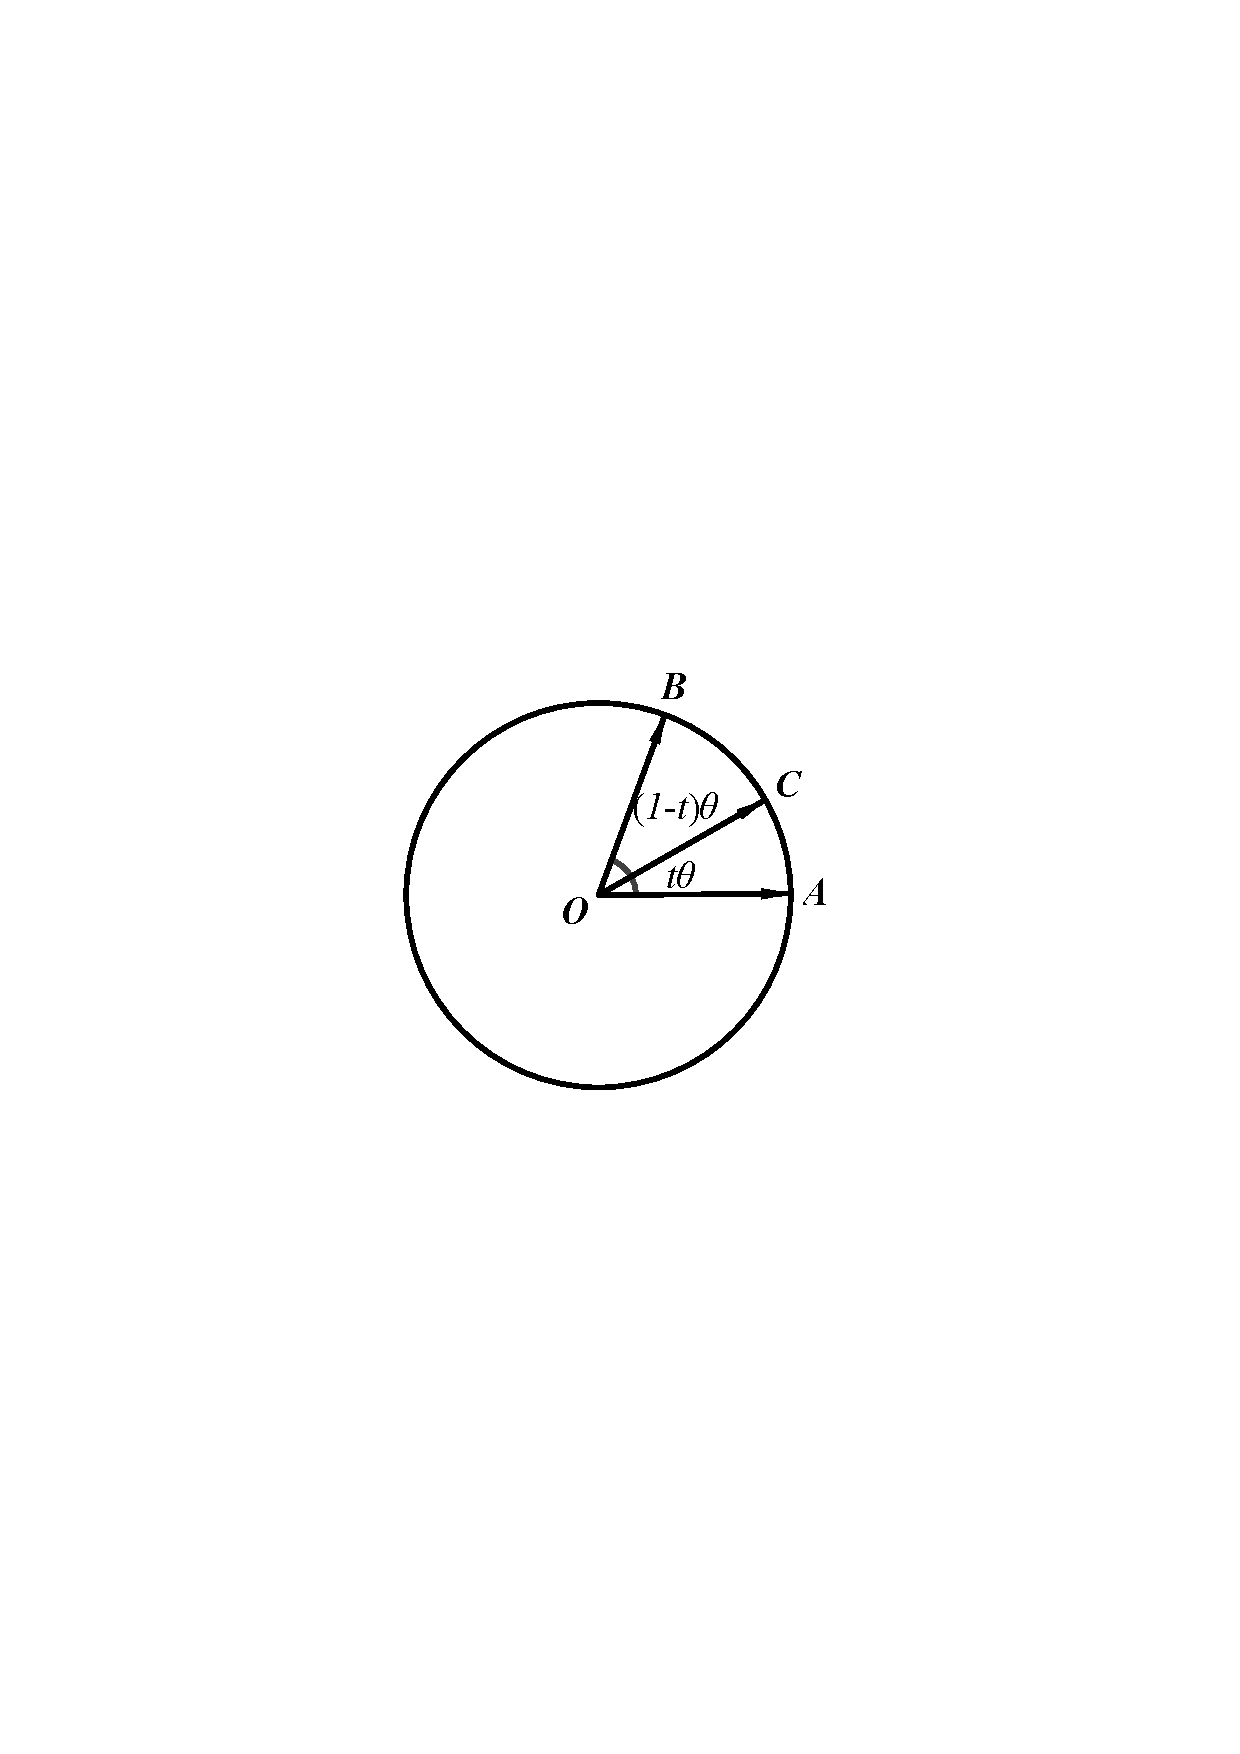
\includegraphics[width=0.4\linewidth]{单位圆上3个向量v1v2合成v四元数背景}
\end{figure} 

\subsection{解三角形}
\item 外心:三条\underline{\ \ifte 中垂\else \hspace{1.5cm} \fi\ }线的交点;\\
内心:三条\underline{\ \ifte 角平分\else \hspace{1.5cm} \fi\ }线的交点;\\
重心:三条\underline{\ \ifte 中\else \hspace{1.5cm} \fi\ }线的交点;\\
垂心:三条\underline{\ \ifte 垂\else \hspace{1.5cm} \fi\ }线的交点。

\item 对于$ \Delta ABC $,重心$ G $分割中线的比例为
\underline{\ \ifte 1:2\else \hspace{1cm} \fi\ }. \\
设$ O $为空间中的任意一点,则
\begin{align*}
    \vec{OG}=\underline{\ \ifte \dfrac{1}{3}
    \else \hspace{1cm} \fi\ } (\vec{OA}+\vec{OB}+\vec{OC})
\end{align*}

\item 正弦定理:
\begin{gather*}
    \underline{\ \ifte \dfrac{a}{\sin A}=\dfrac{b}{\sin B}=
        \dfrac{c}{\sin C} =2R \else \hspace{5cm} \fi\ }
\end{gather*}
$ R $为三角形外接圆半径。

\item 余弦定理:
\begin{align*}
    c^2 &=a^2+b^2-2\vec{a}\cdot\vec{b} \\
        &=\underline{\ \ifte a^2+b^2-2ab\cos C
          \else \hspace{2cm} \fi\ }  \\
    \vec{a}\cdot\vec{b} &=\underline{\ \ifte 
    \dfrac{a^2+b^2-c^2}{2} \else \hspace{2cm} \fi\ } \\
    \cos C &=\underline{\ \ifte 
        \dfrac{a^2+b^2-c^2}{2ab} \else \hspace{2cm} \fi\ }
\end{align*}

\item 对任意三角形,“大边”是”大角”的充要条件。

\item $^*$ 对于$ \Delta ABC $,
\begin{align*}
    a+b+c\geq 2(a\cos A+b\cos B+ c\cos C)
\end{align*}
将三个余弦定理的式子相加可得:
\begin{gather*}
    a^2+b^2+c^2=2bc\cos A+2ac\cos B+ 2ab\cos C
\end{gather*}
将上式中的$ a,b,c $换成任意实数$ x,y,z $,
同时保持$ A+B+C=\pi $,那么有嵌入不等式
\begin{align*}
    x^2+y^2+z^2 \geq \underline{\ \ifte 2yz\cos A+
    2zx\cos B + 2xy\cos C\else \hspace{4cm} \fi\ }
\end{align*}

\item $ (a^2-b^2)^2+(2ab)^2=(\underline{\ \ifte a^2+b^2
    \else \hspace{1cm} \fi\ })^2 $,具有勾股定理的形式。
让$ a,b (a\neq b) $取正整数,就能得到勾股数,比如 
 (3,4,5), (5,12,13), (7,24,25), (8,15,17), 
 (9,40,41), (11,60,61), (20,21,29).

\item 把上一条中的$ a^2 $换成$ \vec{a} $,$ b^2 $换成$ \vec{b} $,
实数乘法换成向量点乘,就得到向量的极化恒等式:
\begin{gather*}
    \underline{\ \ifte 4 \vec{a}\cdot \vec{b}=
    (\vec{a}+\vec{b})^2-(\vec{a}-\vec{b})^2\else \hspace{6cm} \fi\ }
\end{gather*}

\item 对于$ \Delta ABC $,$ R $为外接圆半径,$ r $为内切圆半径,
$ p=\dfrac{a+b+c}{2} $为三角形周长的一半,三角形的面积公式有:\\
两边夹角:\underline{\ \ifte $ \dfrac{1}{2}ab\sin C=\dfrac{1}{2}
bc\sin A=\dfrac{1}{2}ac\sin B $\else \hspace{4.5cm} \fi\ }. \\
只含$ R,A,B,C $:\underline{\ \ifte 
$ 2R^2\sin A\sin B\sin C $\else \hspace{2cm} \fi\ }. \\
只含$ R,a,b,c $:\underline{\ \ifte 
$ \dfrac{abc}{4R} $\else \hspace{2cm} \fi\ }. \\
只含$ p,r $:\underline{\ \ifte $ pr $\else \hspace{2cm} \fi\ }.\\
只含$ p,a,b,c $:\underline{\ \ifte 
$ \sqrt{p(p-a)(p-b)(p-c)} $\else \hspace{4cm} \fi\ }. 

\item $ r $为内切圆半径,则$ r=\underline{\ \ifte 
    \sqrt{\frac{(p-a)(p-b)(p-c)}{p}}\else \hspace{2cm} \fi\ } $
\ifte \else (用$ p,a,b,c $表示)\fi.

\item $^*$ 对于$ \Delta ABC $,外森比克不等式:
\begin{gather*}
    a^2+b^2+c^2 \geq \underline{\ \ifte 
        4\sqrt{3}\else \hspace{1cm} \fi\ }S_{\Delta ABC} 
\end{gather*}

\item $^*$ $ \Delta ABC $的\underline{费马点}:分别以
$ AB,BC,AC $为边,在$ \Delta ABC $外部(或内部)作三个等边三角形,
这三个等边三角形的外接圆会交于同一点,即费马点。当三角形的最大内角
小于$ 120^{\circ} $时,费马点位于三角形内部,设费马点与三个顶点
连线长度分别为$ x,y,z $,则
\begin{gather*}
    xy+yz+zx=\dfrac{4}{\sqrt{3}}S_{\Delta ABC}\leq 
    \dfrac{1}{3}(a^2+b^2+c^2)
\end{gather*}

\item $^*$ 三角形的内心和外心的距离为$ \sqrt{R(R-2r)} $.\\
任意三角形的外接圆半径大于等于2倍内切圆半径($ R\geq2r $).

\item $^*$ $ \Delta ABC $内部有任意一点$ O $,
记$ \Delta AOB $,$ \Delta BOC $,$ \Delta COA $
的面积分别为$ S_C,S_A,S_B $,那么有:
\begin{align*}
    S_A\cdot \underline{\ \ifte \vec{OA}
        \else \hspace{0.5cm} \fi\ }+ 
    S_B\cdot \underline{\ \ifte \vec{OB}
        \else \hspace{0.5cm} \fi\ }+
    S_C\cdot \underline{\ \ifte \vec{OC}
        \else \hspace{0.5cm} \fi\ }= \vec{0}
\end{align*}
$\diamond$ 当$ O $是$ \Delta ABC $的重心时,
\begin{gather*}
    S_A:S_B:S_C=\underline{\ \ifte 1:1:1
        \else \hspace{3cm} \fi\ }
\end{gather*}
$\diamond$ 当$ O $是$ \Delta ABC $的垂心时,
\begin{gather*}
    S_A:S_B:S_C=\underline{\ \ifte \tan A:
    \tan B:\tan C\else \hspace{3cm} \fi\ } 
\end{gather*}
$\diamond$ 当$ O $是$ \Delta ABC $的内心时,
\begin{gather*}
    S_A:S_B:S_C=\underline{\ \ifte a:b:c
        \else \hspace{3cm} \fi\ }
\end{gather*}
$\diamond$ 当$ O $是$ \Delta ABC $的外心时,
\begin{gather*}
    S_A:S_B:S_C=\underline{\ \ifte 
        \sin 2A:\sin 2B:\sin 2C
        \else \hspace{3cm} \fi\ }
\end{gather*}

\item $ D $是$ \Delta ABC $的$ BC $边上的一点,则
$ \dfrac{|AB|}{|AC|}=\dfrac{|BD|}{|CD|} $的充分必要条件是:
$ AD $是\underline{\ \ifte $ \angle BAC $的角平分线
    \else \hspace{4cm} \fi\ }。
\begin{figure}[H]
    \centering
    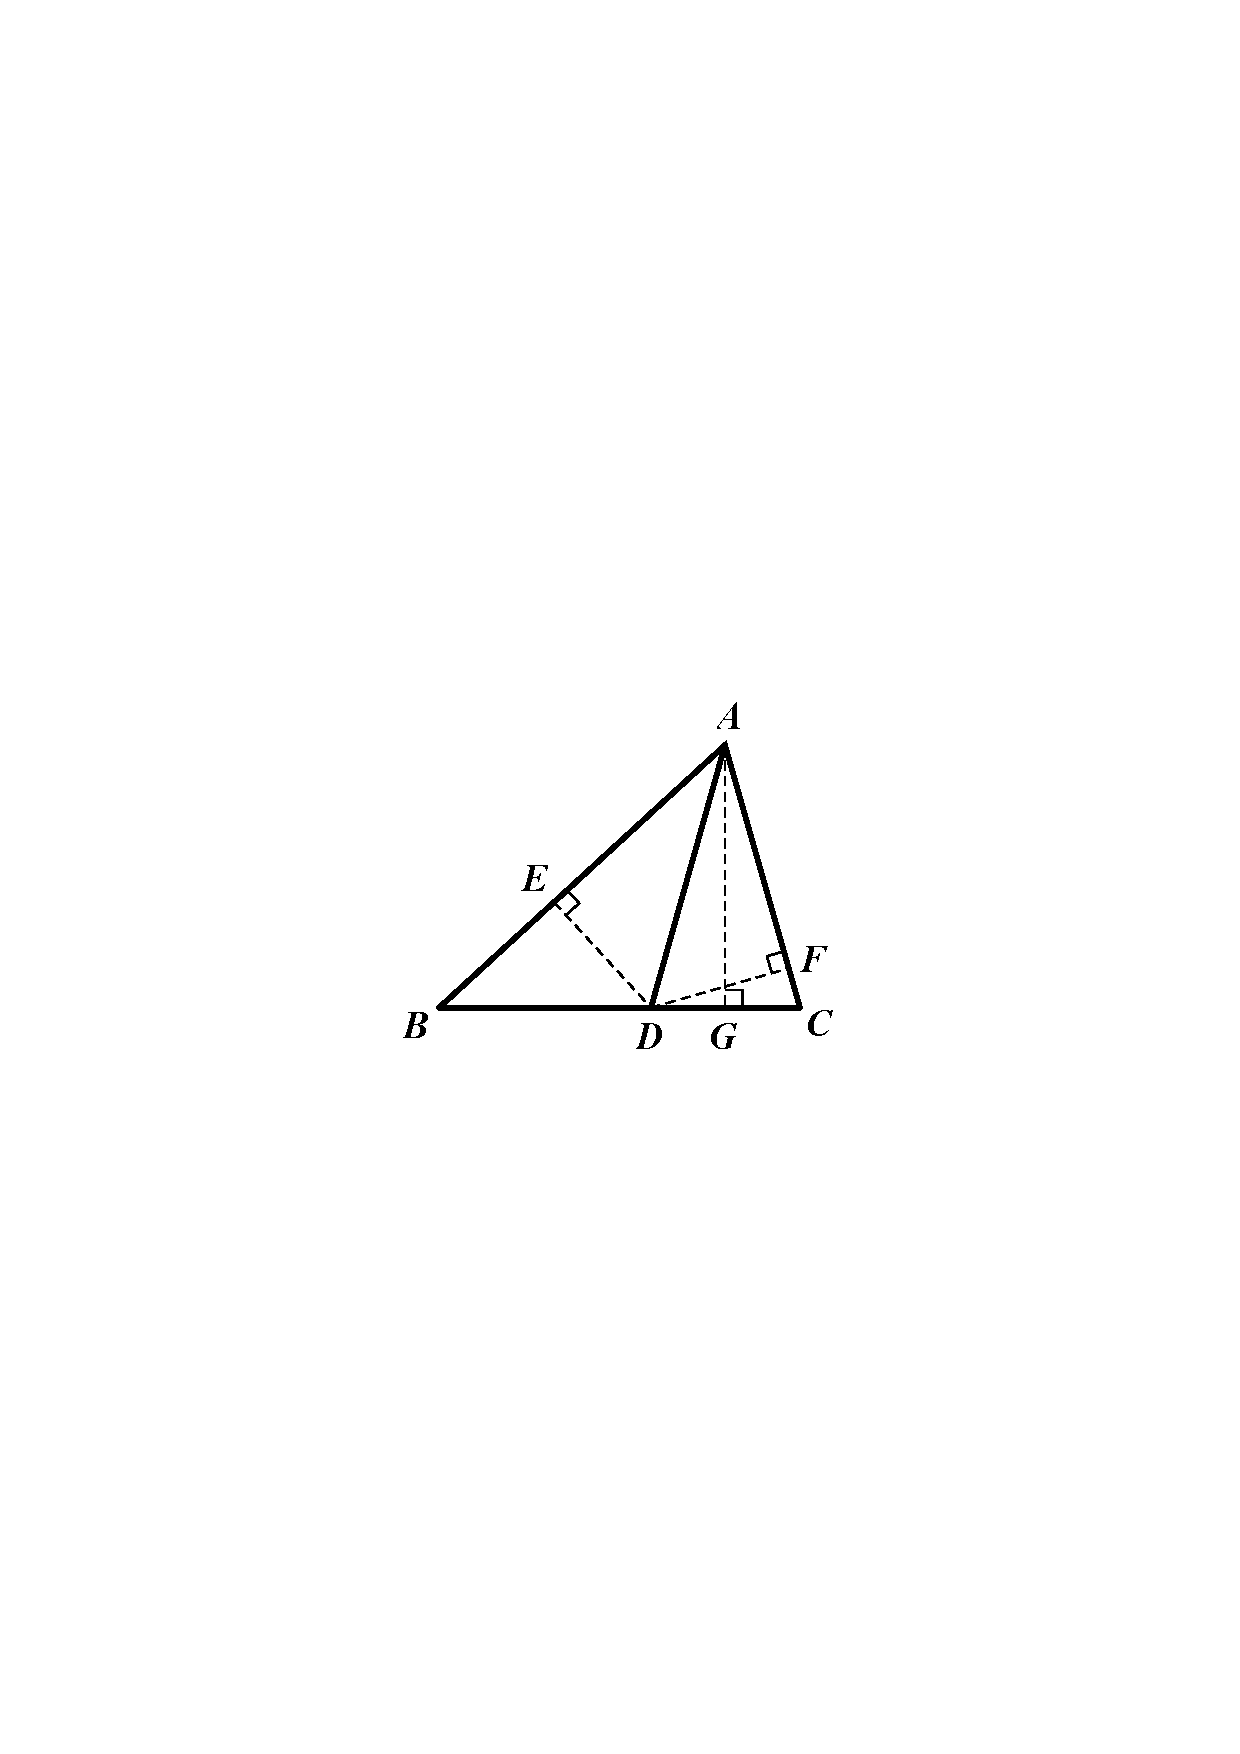
\includegraphics[width=0.4\linewidth]{三角形的内角平分线定理}
\end{figure}

\item (皮克公式)横纵坐标均为整数的点称为格点,所有顶点均在格点的
多边形称为格点多边形。设格点多边形内部有$ N $个格点,
边界上有$ B $个格点。则多边形的面积为
\underline{\ \ifte $ N+\dfrac{B}{2}-1 $
    \else \hspace{3cm} \fi\ }.

\subsection{导数与积分}

\item 基本初等函数的导数公式:\\
$ (x^{\alpha})'=\underline{\ \ifte \alpha x^{\alpha-1}
    \else \hspace{2cm} \fi\ } $,\\
$ (\ln x)'=\underline{\ \ifte \dfrac{1}{x}\else \hspace{2cm} \fi\ } $,\\
$ (a^x)'=\underline{\ \ifte (\ln a) a^x\else \hspace{2cm} \fi\ } $,\\
$ (\e^x)'=\underline{\ \ifte \e^x\else \hspace{2cm} \fi\ } $,\\
$ (\sin x)'=\underline{\ \ifte \cos  x\else \hspace{2cm} \fi\ } $,\\
$ (\cos x)'=\underline{\ \ifte -\sin x\else \hspace{2cm} \fi\ } $,\\
$ (\tan x)'=\underline{\ \ifte \dfrac{1}{\cos ^2 x}
    \else \hspace{2cm} \fi\ } $.

\item 导数运算法则:
\begin{align*}
\left[c_1f(x)+c_2g(x)\right]'&=\underline{\ \ifte 
    c_1f'(x)+c_2g'(x) \else \hspace{3cm} \fi\ } \\
\left[f(x)\cdot g(x) \right]'&= \underline{\ \ifte 
    f'(x)\cdot g(x)+f(x)\cdot g'(x) \else \hspace{3cm} \fi\ } \\
\left[ \dfrac{f(x)}{g(x)}\right]'&=\underline{\ \ifte 
    \dfrac{f'(x)\cdot g(x)-f(x)\cdot g'(x)}{g^2(x)}
    \else \hspace{3cm} \fi\ }
\end{align*}

\item 
\begin{align*}
    \left[f(x)\cdot x^n \right]'&= \underline{\ 
      \ifte x^n f'(x)+nx^{n-1}f(x) \else \hspace{3cm} \fi\ } \\
    \left[ \dfrac{f(x)}{x^n}\right]' &=\underline{\ 
      \ifte \dfrac{xf'(x)-nf(x)}{x^{n+1}} \else \hspace{3cm} \fi\ }
\end{align*}


\item 复合函数求导法则:$ [g(f(x))]'=g'(u)f'(x) $,再将$ u $换回$ f(x) $. 
比如$ [\ln f(x)]'=\underline{\ \ifte \dfrac{f'(x)}{f(x)}
\else \hspace{2cm} \fi\ } $.

\item 设$ f(x)=(x-x_0)^ng(x) $,两边取自然对数,有
\begin{gather*}
    \ln f(x) =n\ln(x-x_0)+\ln g(x)
\end{gather*}
两边求导,有
\begin{align*}
    \frac{f'(x)}{f(x)} =\underline{\ \ifte 
    \frac{n}{x-x_0}+\frac{g'(x)}{g(x)}\else \hspace{3cm} \fi\ }
\end{align*}

\item 可导奇函数的导函数是\underline{\ \ifte 偶\else \hspace{0.5cm} \fi\ }函数
\ifte \else (填“奇”或“偶”)\fi;\\
可导偶函数的导函数是\underline{\ \ifte 奇\else \hspace{0.5cm} \fi\ }函数。

\item 牛顿-莱布尼茨公式(微积分基本公式):
\begin{gather*}
    \int_a^bf'(x)\d x=\underline{\ \ifte 
        f(b)-f(a)\else \hspace{2cm} \fi\ }
\end{gather*}

\item $^*$ 罗必塔(L'Hospital)法则:当$ x\to x_0 $时,如果$ f(x) $和
$ g(x) $均趋于0或$ \pm \infty $,那么
\begin{gather*}
    \lim\limits_{x\to x_0}\dfrac{f(x)}{g(x)}=
    \lim\limits_{x\to x_0}\dfrac{f'(x)}{g'(x)}
\end{gather*}
特别地,$ \lim\limits_{x\to 0} x\ln x=\underline{\ 
    \ifte 0\else \hspace{1cm} \fi\ } $.

\item 把$ \e^x\geq x+1 $中的$ x $换成$ x-1 $,有$ \e^{x-1}\geq x $,
两边同乘$ \e $,有$ \underline{\ \ifte \e^x\geq \e x
    \else \hspace{2cm} \fi\ } $.

\item 把$ \e^x\geq x+1 $中的$ x $换成$ -x $,有$ \e^{-x}\geq -x+1 $,
当$ x<1 $时,两边同时取倒数,有$ \e^x\leq \underline{\ \ifte 
\dfrac{1}{1-x}  \else \hspace{2cm} \fi\ } $.

\item $ x $换成$ \alpha x (\alpha>0)$,有
$ \e^{\alpha x}\geq \alpha x+1 $,当$ 1+\alpha x>0 $时,
两边同时开$ \alpha $次方,有$ \e^x\geq \underline{\ \ifte
(1+\alpha x)^{\frac{1}{\alpha}} \else \hspace{2cm} \fi\ } $. 

\item $^*$ $ \e $是自然对数的底数,$ n\in \textbf{N}^+ $,则
\begin{gather*}
    2 \leq \left( 1+\dfrac{1}{n}\right)^{n} < \e < 
    \left( 1+\dfrac{1}{n}\right)^{n+1}
\end{gather*}

\item 对于三次函数$ y=f(x)=ax^3+bx^2+cx+d $,对称中心的坐标为
\underline{\ \ifte $ \left(-\dfrac{b}{3a},f\Big(-\dfrac{b}{3a}
    \Big)\right) $\else \hspace{2.5cm} \fi\ },
对称中心也是三次函数的拐点(二阶导数为0,且二阶导数在此点左右异号)。

\item $^*$ 对任意$ n $次首一多项式$ P(x) $(最高次项系数为1的多项式),设$ M $代表
$ |P(x)| $在区间$ [-1,1] $上的最大值,那么无论其它项的系数怎么变化(保持首一),
$ M $总是大于等于\underline{\ \ifte $ \dfrac{1}{2^{n-1}} $
    \else \hspace{2cm} \fi\ }. 

\item $^*$ 函数$ f(x) $在$ x=x_0 $处的泰勒(Taylor)级数
\begin{gather*}
    f(x)=f(x_0)+\dfrac{f'(x_0)}{1!}(x-x_0)+\dfrac{f''(x_0)}{2!}
    (x-x_0)^2\\ + \dfrac{f'''(x_0)}{3!}(x-x_0)^3+\cdots+
    \dfrac{f^{(n)}(x_0)}{n!}(x-x_0)^n+\cdots
\end{gather*}
当$ x_0=0 $时,
\begin{align*}
    \e^x=&\ \underline{\ \ifte 1+x+\dfrac{x^2}{2!}+\cdots
        +\dfrac{x^n}{n!}\else \hspace{4cm} \fi\ }+\cdots \\
    \sin x=&\ x-\dfrac{x^3}{3!}+\dfrac{x^5}{5!}-\cdots +(-1)^n
    \dfrac{x^{2n+1}}{(2n+1)!} +\cdots \\
    \cos x=&\ 1-\dfrac{x^2}{2!}+\dfrac{x^4}{4!}-\cdots +(-1)^n
    \dfrac{x^{2n}}{(2n)!} +\cdots \\
    \sqrt{1+x}=&\ 1+\dfrac{1}{2}x-\dfrac{1}{2\cdot 4}x^2
    +\dfrac{1\cdot 3}{2\cdot 4\cdot 6}x^3-\cdots \\
    \ln(1+x)=&\ x-\dfrac{x^2}{2}+\dfrac{x^3}{3}-\dfrac{x^4}{4}+
    \cdots (-1)^{n-1}\dfrac{x^n}{n}+ \cdots \\
    \ln\dfrac{1+x}{1-x}=&\ 2\left(\underline{\ \ifte 
    x+\dfrac{x^3}{3}+\dfrac{x^5}{5}+\cdots +
    \dfrac{x^{2n-1}}{2n-1}\else \hspace{3cm} \fi\ } +\cdots \right)
\end{align*} 

\item 当$ |x| < 0.2 $时,$ \sqrt{1+x}\approx 1+\dfrac{1}{2}x $\ ($ x $可正可负).
而且$ |x| $越小,这个估算公式越精确。\\
$ \sqrt{1.1}=1.048808\cdots \approx 1+\dfrac{1}{2}\times 0.1=1.05 $,\\
$ \sqrt{73}=8.544003\cdots=\sqrt{64+9}=\sqrt{64\left(1+\dfrac{9}{64}\right)}=$\\ 
\ifte \underline{ {\footnotesize $ 8\sqrt{1+\dfrac{9}{64}}\approx 8\left(1+
\dfrac{9}{2\times 64}\right)=8+\dfrac{9}{2\times 8}=8\dfrac{9}{16} $} }
\else\\ \underline{\ \hspace{6cm} }\fi .

\item 拉格朗日中值定理: 如果函数$ f(x) $满足:
(1)在闭区间$ [x_1,x_2] $上连续;
(2)在开区间$ (x_1,x_2) $内可导。\\
那么至少存在一点$ \xi\in(x_1,x_2) $,
使得$ f'(\xi)=\dfrac{f(x_2)-f(x_1)}{x_2-x_1} $.
(至少能作出一条和割线斜率相等的切线)。 

\item $^*$ 厄米特-哈达玛(Hermite-Hadamard)不等式:
$ f(x) $在区间$ [a,b] $上连续且可积,$ \forall x_1,x_2\in [a,b],\ 
x_1<x_2 $,如果$ f\Big(\dfrac{x_1+x_2}{2}\Big)<
\dfrac{1}{2}[f(x_1)+f(x_2)] $(等价于$ f''(x)>0 $),那么有 
\begin{align*}
    f\left(\dfrac{x_1+x_2}{2}\right) &<\dfrac{1}{x_2-x_1}
    \int_{x_1}^{x_2}f(x)\d x \\ 
    &< \dfrac{f(x_1)+f(x_2)}{2}
\end{align*}

\item $^*$ 小于等于$ n $的全部正整数的$ 1\sim 5 $次方的求和结果:
\begin{align*}
    & 1^1+2^1+3^1+\cdots +n^1=\dfrac{n^2}{2}+\dfrac{n}{2}\\
    & 1^2+2^2+3^2+\cdots +n^2=\dfrac{n^3}{3}+
        \dfrac{n^2}{2}+\dfrac{n}{6}\\
    & 1^3+2^3+3^3+\cdots +n^3=\dfrac{n^4}{4}+
        \dfrac{n^3}{2}+\dfrac{n^2}{4} \\
    & 1^4+2^4+3^4+\cdots +n^4=\dfrac{n^5}{5}+\dfrac{n^4}{2}
        +\dfrac{n^3}{3}-\dfrac{n}{30} \\
    & 1^5+2^5+3^5+\cdots +n^5=\dfrac{n^6}{6}+\dfrac{n^5}{2}
        +\dfrac{5n^4}{12}-\dfrac{n^2}{12} 
\end{align*}
$ 1\sim n $的$ k $次方求和结果是关于$ n $的$ k+1 $次多项式,
多项式的系数从高次项到低次项依次为
\begin{gather*}
    \dfrac{1}{k+1},\ \dfrac{1}{2},\ \dfrac{k}{12},\ 0,
    \ -\dfrac{k(k-1)(k-2)}{720},\cdots
\end{gather*}
以上这些求和公式可以写成如下通式,
\begin{align*}
    &\ 1^k+2^k+3^k+\cdots +n^k  \\=&\ \dfrac{1}{k+1}
    \sum_{j=0}^{k}C_{k+1}^{j}B_{j}n^{k+1-j}+n^{k} \\
    =&\ \dfrac{1}{k+1}n^{k+1}+\dfrac{1}{2}n^k+\dfrac{k}{12}n^{k-1}+\cdots
\end{align*}
$ B_j $为伯努利数,$ B_0=1 $,\ $ B_1=-\dfrac{1}{2} $,\ 
$ B_2=\dfrac{1}{6}$,\ $B_3=0 $,\ $ B_4=-\dfrac{1}{30}$,\ $B_5=0$,\ $B_6=\dfrac{1}{42}\cdots$
伯努利数满足递推关系:$ 0=\sum\limits_{j=0}^{n-1}C_n^jB_j\ (n\geq 2) $.
以上求和公式实际上是欧拉-麦克劳林求和公式的一个特例。

\item 黎曼zeta函数:$ \zeta(s)=\sum\limits_{n=1}^{\infty} 
\dfrac{1}{n^s}\ (s>1) $,\\ $ \zeta(2)=\sum\limits_{n=1}^{\infty}
\dfrac{1}{n^2}=\underline{\ \ifte \dfrac{\pi^2}{6}
\else \hspace{2cm} \fi\ } $. 
 
\item 非整数次幂求和(只有近似公式,没有精确公式):
\begin{align*}
    &\sum\limits_{l=1}^{n} l^{-1/2}\leq \underline{\ \ifte 
       2n^{1/2}-1 \else \hspace{4cm} \fi\ }  \\  
    &\sum\limits_{l=1}^{n} l^{-1/3}\leq \underline{\ \ifte 
      \dfrac{3}{2}n^{2/3}-\dfrac{1}{2} \else \hspace{4cm} \fi\ }  \\ 
    &\sum\limits_{l=1}^{n} l^{1/3}\leq \underline{\ \ifte 
       \dfrac{3}{4}n^{4/3}+\dfrac{1}{2}n^{1/3}-\dfrac{1}{4}
       \else \hspace{4cm} \fi\ }  \\
    &\sum\limits_{l=1}^{n} l^{1/2}\leq \underline{\ \ifte 
        \dfrac{2}{3}n^{3/2} +\dfrac{1}{2}n^{1/2}-
        \dfrac{1}{6} \else \hspace{4cm} \fi\ }
\end{align*}
系数的规律与整数次幂的规律相同,只是不要出现负幂项。
常数项的作用是提高近似公式的精度,可通过令$ n=1 $来确定常数项。

\subsection{不等式}

\item 糖水不等式:若$ 0<b<a,c>0 $,则\\
$ \dfrac{b}{a}<
\underline{\ \ifte \dfrac{b+c}{a+c}\else \hspace{1.5cm} \fi\ } $ .\\
$\dfrac{1}{a^k-1}\leq \underline{\ \ifte 
\dfrac{1+1}{a^k-1+1}=\dfrac{2}{a^{k}} \else \hspace{4cm} \fi\ } $ .

\item 设$ a,b,c,d $均大于0,且$ \dfrac{a}{b}<\dfrac{c}{d} $,
那么 \\ $ \dfrac{a}{b}<\dfrac{a+c}{b+d}<\dfrac{c}{d} $. 

\item $ a,b\in\mathbf{R} $,则\\ $ \dfrac{|a+b|}{1+|a+b|} $ 
\underline{\ \ifte $ \leq $ \else \hspace{1cm} \fi\ } 
 $ \dfrac{|a|}{1+|a|}+\dfrac{|b|}{1+|b|} $. \\ 
 (填$ <,>,\leq,\geq $之一。)

\item 设$ a>1 $,当$ k\geq 1 $时,$ a^k-1\geq a^k-a^{k-1}=(a-1)a^{k-1}$,所以
\begin{gather*}
    \dfrac{1}{a^k-1}\leq \underline{\ \ifte 
    \dfrac{1}{(a-1)a^{k-1}} \else \hspace{2cm} \fi\ }
\end{gather*}

\item 伯努利不等式:当$ x>-1 $时,\\
$ \bullet $ 若$ \alpha>1 $,则 $ (1+x)^{\alpha} \underline{\ 
    \ifte \geq \else \hspace{0.5cm} \fi\ } 1+\alpha x  $;\\
$ \bullet $ 若$ 0<\alpha<1 $,则 $ (1+x)^{\alpha} \underline{\ 
    \ifte \leq \else \hspace{0.5cm} \fi\ } 1+\alpha x $. \\
用数学归纳法或求导证明。

\item $^*$ 广义伯努利不等式:\\
若$ x_1,x_2,\cdots x_n >0, n\geq 2 $,则
\begin{align*}
     &\ (1+x_1)(1+x_2)\cdots (1+x_n)\\
    >&\ 1+(x_1+x_2+\cdots +x_n) 
\end{align*}
若$ x_1,x_2,\cdots x_n \in (0,1), n\geq 2 $,则
\begin{align*}
     &\ (1-x_1)(1-x_2)\cdots (1-x_n)\\
    >&\ 1-(x_1+x_2+\cdots +x_n) 
\end{align*}
用数学归纳法证明。

\item $ x\in \left( 0,\dfrac{\pi}{2}\right) $,
\begin{gather*}
    \underline{\ \ifte \dfrac{2}{\pi}x\else \hspace{0.5cm} \fi\ }
    <\sin x < \underline{\ \ifte x\else \hspace{0.5cm} \fi\ } <
    \\ x+\dfrac{x^3}{3} 
    <\dfrac{3x}{3-x^2}<\tan x <\dfrac{x}{1-\frac{2}{\pi}x}
\end{gather*} 

\item $^*$ $ x\in (0,1) $,
\begin{gather*}
    \dfrac{x}{\sqrt{1+x^2}}<\dfrac{x}{\sqrt{1+\frac{2}{3}x^2}}<
    \sin x<\dfrac{x}{\sqrt{1+\frac{1}{3}x^2}}<x \\
     <\dfrac{x}{\sqrt{1-\frac{1}{3}x^2}}<
    \tan x<\dfrac{x}{\sqrt{1-\frac{2}{3}x^2}}<
    \dfrac{x}{\sqrt{1-x^2}}
\end{gather*} 

\item $ x\in \textbf{R} $,$ \cos x\geq \underline{\ 
    \ifte 1-\dfrac{1}{2}x^2 \else \hspace{2cm} \fi\ } $(泰勒级数取前两项). \\
$ x\in \left(0,\dfrac{\pi}{2}\right) $,$ \cos x <1-\dfrac{4x^2}{\pi^2} $. 

\item $ x\in (0,1) $,$ \e^{2x}<\dfrac{1+x}{1-x} $. \\
两边取自然对数,有$ 2x<\underline{\ \ifte 
    \ln\dfrac{1+x}{1-x} \else \hspace{1cm} \fi\ } $. \\
令$ t=\dfrac{1+x}{1-x}\in(1,+\infty) $,则$ x=\underline{\ \ifte 
    \dfrac{t-1}{t+1}\else \hspace{1cm} \fi\ } $,
上面的不等式变为$ \underline{\ \ifte \dfrac{2(t-1)}{t+1}<\ln t
    \else \hspace{2cm} \fi\ } $.

\item $ t\in(1,+\infty) $,$ \ln t<\underline{\ \ifte 
    \sqrt{t}-\dfrac{1}{\sqrt{t}} \else \hspace{2cm} \fi\ } $
\ifte \else (含$ \sqrt{t} $) \fi.

\item 对任意两个不等的正实数$ x_1,x_2 $,有
\begin{align*}
    \sqrt{x_1x_2}<\dfrac{x_2-x_1}{\ln x_2-\ln x_1}<\dfrac{x_1+x_2}{2}
\end{align*}
$ \dfrac{x_2-x_1}{\ln x_2-\ln x_1} $称为对数平均值。
把上式中的$ x_1 $换成$ \e^{x_1} $,$ x_2 $换成$ \e^{x_2} $,可得:
\begin{align*}
    \underline{\ \ifte\e^{\frac{x_1+x_2}{2}}<\dfrac{\e^{x_2}
    -\e^{x_1}}{x_2-x_1}<\dfrac{\e^{x_1}+\e^{x_2}}{2}
    \else \hspace{7cm} \fi\ }
\end{align*}

\item 两变量均值不等式\ifte \else (包含4种均值) \fi:
\begin{align*}
    \underline{\ \ifte \dfrac{2}{\dfrac{1}{a}+\dfrac{1}{b}}\leq 
    \sqrt{ab} \leq \dfrac{a+b}{2}
    \leq \sqrt{\dfrac{a^2+b^2}{2}}\else \hspace{7cm} \fi\ }
\end{align*}

\item $^*$ 将上式推广到$ n $变量情形:\\
调和均值$(H_n) \leq $几何均值$(G_n) \leq $ \\
算术均值$(A_n) \leq $平方均值$ (Q_n) $
\begin{gather*}
    \dfrac{n}{\dfrac{1}{a_1}+\dfrac{1}{a_2}+\cdots +\dfrac{1}{a_n}}\leq 
    \sqrt[n]{a_1a_2\cdots a_n} \leq \\ \dfrac{a_1+a_2+\cdots +a_n}{n} \leq 
    \sqrt{\dfrac{a_1^2+a_2^2+\cdots +a_n^2}{n}}
\end{gather*}
其中,$ a_1,a_2,\cdots a_n $均非负。

\item 给定$ \lambda a+\mu b=C $,求$ ab $的最大值和$ \dfrac{k_1}{a}+
\dfrac{k_2}{b} $的最小值。其中,$ \lambda,\mu,C,k_1,k_2 $为正的常数,
$ a,b $为正的变量。
\begin{gather*}
    ab=\dfrac{1}{\lambda\mu}(\lambda a\cdot \mu b)\leq 
   \underline{\ \ifte \dfrac{1}{\lambda\mu}\left(\dfrac{\lambda a
   +\mu b}{2}\right)^2=\dfrac{C^2}{4\lambda\mu}\else \hspace{4cm} \fi\ } 
\end{gather*}
\begin{align*}
    \dfrac{k_1}{a}+\dfrac{k_2}{b} &=\left(\dfrac{k_1}{a}+
    \dfrac{k_2}{b}\right)\cdot
    \dfrac{1}{C}\left(\lambda a+\mu b\right)\\ &=\underline{\ \ifte 
    \dfrac{1}{C}\left(k_1\lambda +k_2\mu +k_1\mu \dfrac{b}{a}+k_2
    \lambda \dfrac{a}{b}\right)\else \hspace{4cm} \fi\ } 
\end{align*}

\item 若$ x\in \textbf{R} $,则$ \sqrt{x^2+4}+\dfrac{1}{\sqrt{x^2+4}}
\geq \underline{\ \ifte \dfrac{5}{2}\else \hspace{1cm} \fi\ } $.

\item $^*$ 加权算术-几何均值不等式:正数$ \lambda_k $满足$ \lambda_1+
\lambda_2+\cdots +\lambda_n=1 $,且 $ x_k\geq 0 $,那么
\begin{align*}
    x_1^{\lambda_1}x_2^{\lambda_2}\cdots x_n^{\lambda_n}\leq 
    \lambda_1x_1+\lambda_2x_2+\cdots +\lambda_nx_n
\end{align*}

\item 柯西不等式:\\ $ \vec{a}=(a_1,a_2,\cdots,a_n),
\vec{b}=(b_1,b_2,\cdots,b_n) $,那么
\begin{gather*}
    |\vec{a}\cdot \vec{b}|
    =|\vec{a}||\vec{b}||\cos\theta|\leq 
    |\vec{a}||\vec{b}| \\
    |\vec{a}\cdot \vec{b}|^2 \leq 
    |\vec{a}|^2|\vec{b}|^2 
\end{gather*}
把上式转化为坐标表示:
\begin{gather*}
    \underline{\ \ifte \left( \sum_{k=1}^{n}a_kb_k\right)^2 
    \leq \left(\sum_{k=1}^{n}a_k^2\right) 
    \left(\sum_{k=1}^{n}b_k^2 \right) \else \hspace{5cm} \fi\ }
\end{gather*}

\item $ a,b,c\in \textbf{R} $,因为$ (a-b)^2+(b-c)^2+(c-a)^2\geq 0 $,所以,
$ a^2+b^2+c^2\geq \underline{\ \ifte ab+bc+ca\else \hspace{2cm} \fi\ } $.

\item $^*$ 赫尔德(Hölder)不等式:$ p>1,q>1,\dfrac{1}{p}+\dfrac{1}{q}=1 $,
$ a_k\geq 0,b_k\geq 0,k=1,2\cdots n $,那么
\begin{gather*}
    \sum_{k=1}^{n}a_kb_k\leq \left(\sum_{k=1}^{n}a_k^p\right)^{\frac{1}{p}}
    \cdot\left(\sum_{k=1}^{n}b_k^q\right)^{\frac{1}{q}}
\end{gather*}
等号成立的条件是:存在非0实数$ \lambda $,对任意$ k=1,2\cdots n $都有
$ \lambda a_k=b_k $. 当$ p=q=2 $时,就变成柯西不等式。

\item $^*$ 闵可夫斯基(Minkowski)不等式:$ r>0,r\neq 1,a_k>0,b_k>0 $,那么
{\scriptsize \begin{align*}
    \left[\sum_{k=1}^{n}(a_k+b_k)^r\right]^{\frac{1}{r}}\leq
    \left(\sum_{k=1}^{n}a_k^r\right)^{\frac{1}{r}}+
    \left(\sum_{k=1}^{n}b_k^r\right)^{\frac{1}{r}} \quad(r>1) \\
    \left[\sum_{k=1}^{n}(a_k+b_k)^r\right]^{\frac{1}{r}}\geq
    \left(\sum_{k=1}^{n}a_k^r\right)^{\frac{1}{r}}+
    \left(\sum_{k=1}^{n}b_k^r\right)^{\frac{1}{r}} \quad(r<1)
\end{align*} }
以上两式等号成立的条件都是:存在非0实数$ \lambda $,对任意$ k=1,2\cdots n $都有
$ \lambda a_k=b_k $. 

\item 含根号的缩放:
\begin{gather*}
    \underline{\ \ifte \sqrt{k+1}+\sqrt{k}\else \hspace{2cm} \fi\ }
    >2\sqrt{k}>\underline{\ \ifte \sqrt{k+\dfrac{1}{2}}+
    \sqrt{k-\dfrac{1}{2}} \else \hspace{2cm} \fi\ }> \\
    \underline{\ \ifte \sqrt{k+1}+\sqrt{k-1}\else \hspace{2cm} \fi\ }
    >\underline{\ \ifte \sqrt{k}+\sqrt{k-1}\else \hspace{2cm} \fi\ }
\end{gather*}
以上各项除$ 2\sqrt{k} $外,取倒数后均可裂项。

\item 含平方的缩放:
\begin{gather*}
    \underline{\ \ifte k(k+1)\else \hspace{2cm} \fi\ }\geq k^2+1>k^2>
    \underline{\ \ifte \left( k-\dfrac{1}{2}\right)\left(k+
    \dfrac{1}{2}\right)\else \hspace{2cm} \fi\ } \\
    >\underline{\ \ifte (k-1)(k+1)\else \hspace{2cm} \fi\ } \geq
    \underline{\ \ifte k(k-1)\else \hspace{2cm} \fi\ }
\end{gather*}
以上各项除$ k^2+1 $和$ k^2 $外,取倒数后均可裂项。

\item 正整数倒数求和缩放:
\begin{gather*}
    \underline{\ \ifte \ln(n+1)\else \hspace{1.6cm} \fi\ }
    <\dfrac{1}{1}+\dfrac{1}{2}+\cdots +\dfrac{1}{n}
    <\underline{\ \ifte 1+\ln n\else \hspace{1.6cm} \fi\ }
\end{gather*}

\subsection{数列}
\item 设$ \{a_n \} $ 是公差为$ d $的等差数列,$ S_n $是其前$ n $项和,
\begin{itemize}[leftmargin=-4pt]
\item 若$ m+n=s+t $,则$ a_m+a_n=\underline{\ \ifte 
    a_s+a_t\else \hspace{2cm} \fi\ } $;
\item $ S_{m+n}=S_m+S_n+\underline{\ \ifte mnd
    \else \hspace{1cm} \fi\ } $;
\item $ \dfrac{S_{2n-1}}{a_n}=\underline{\ \ifte 2n-1
    \else \hspace{2cm} \fi\ } $;
\item $ m\neq n $,$ \dfrac{S_m-S_n}{m-n}=\dfrac{S_{m+n}}{m+n}=
    \underline{\ \ifte \dfrac{d}{2}(m+n)+(a_1-\dfrac{d}{2})
    \else \hspace{2cm} \fi\ } $;
\item $ S_n,S_{2n}-S_n,S_{3n}-S_{2n} \cdots $是公差为
\underline{\ \ifte $ n^2d $\else \hspace{0.5cm} \fi\ }的等差数列;

\item 在前$ 2n $项中,\\ $ \dfrac{\text{奇数项之和}}{\text{偶数项之和}} = 
\dfrac{a_1+a_3+\cdots+a_{2n-1}}{a_2+a_4+\cdots+a_{2n}} 
=\underline{\ \ifte \dfrac{a_n}{a_{n+1}} \else \hspace{1cm} \fi\ } $;

\item 在前$ 2n+1 $项中,\\ $ \dfrac{\text{奇数项之和}}{\text{偶数项之和}}= 
\dfrac{a_1+a_3+\cdots+a_{2n+1}}{a_2+a_4+\cdots+a_{2n}}=
\underline{\ \ifte \dfrac{n+1}{n} \else \hspace{1cm} \fi\ } $;
\end{itemize}

\item 等比数列$ a_n=a_1x^{n-1} $的求和公式:当$ x\neq 1 $时,$ S_n=
\underline{\ \ifte \dfrac{a_1(1-x^n)}{1-x}=\dfrac{a_1-a_{n+1}}{1-x}
    \else \hspace{4cm} \fi\ } $. 若$ |x|<1 $,则
$ \sum\limits_{k=0}^{\infty} x^{k}=\underline{\ \ifte 
    \dfrac{1}{1-x}\else \hspace{2cm} \fi\ } $.

\item 等差乘以等比型数列求和($ x\neq 1 $):
\begin{gather*}
    \sum_{k=1}^{n}kx^{k-1}=\dfrac{nx^{n+1}-(n+1)x^n+1}{(1-x)^2}
\end{gather*}
当$ |x|<1 $时,
\begin{gather*}
    \sum_{k=1}^{\infty} kx^{k-1}=\underline{\ \ifte 
        \dfrac{1}{(1-x)^2} \else \hspace{2cm} \fi\ }
\end{gather*}
对上式求导,
\begin{gather*}
    \sum_{k=2}^{\infty} k(k-1)x^{k-2}=\underline{\ \ifte 
    \dfrac{2}{(1-x)^3} \else \hspace{2cm} \fi\ }
\end{gather*}
因为$ k^2x^{k-1}=x\cdot k(k-1)x^{k-2}+kx^{k-1} $,所以
\begin{align*}
    \sum_{k=1}^{\infty} k^2x^{k-1}=&\ \underline{\ 
        \ifte \dfrac{1+x}{(1-x)^3}\else \hspace{2cm} \fi\ } \\
    \sum_{k=1}^{\infty} k^2x^{k}=&\ \underline{\ \ifte 
        \dfrac{x(1+x)}{(1-x)^3} \else \hspace{2cm} \fi\ }
\end{align*}

\item 常见裂项方法:
{\footnotesize \begin{align*}
    &\dfrac{1}{n(n+k)}=\underline{\ \ifte 
        \dfrac{1}{k}\left(\dfrac{1}{n}-\dfrac{1}{n+k} \right)
        \else \hspace{4cm} \fi\ } \\
    &\dfrac{1}{n(n+1)(n+2)}=\underline{\ \ifte \dfrac{1}{2} 
        \left[\dfrac{1}{n(n+1)}- \dfrac{1}{(n+1)(n+2)}\right]
        \else \hspace{4cm} \fi\ } \\ 
    &\dfrac{1}{4n^2-1}=\underline{\ \ifte \dfrac{1}{2}
        \left(\dfrac{1}{2n-1}-\dfrac{1}{2n+1} \right)
        \else \hspace{4cm} \fi\ } \\
    &\dfrac{1}{\sqrt{n}+\sqrt{n+k}}=\underline{\ \ifte 
        \dfrac{1}{k}(\sqrt{n+k}-\sqrt{n})
        \else \hspace{4cm} \fi\ } \\ 
    &\dfrac{a^n}{(a^n+1)(a^{n+1}+1)}=\underline{\ \ifte 
        \dfrac{1}{a-1}\left(\dfrac{1}{a^n+1}-
        \dfrac{1}{a^{n+1}+1}\right)\else \hspace{3.5cm} \fi\ }
\end{align*} }

\item $^*$ 阿贝尔(Abel)求和公式:数列$ \{a_n\},\{b_n\} $
的前$ n $项和分别为$ A_n,B_n $,那么
\begin{gather}
    \sum_{k=1}^{n}A_kb_k+\sum_{k=1}^{n-1}a_{k+1}B_k=A_n B_n 
\end{gather}

\item 如果$ f(x) $在区间$ [a,b] $上满足下列2个条件,
则称$ f(x) $为一个压缩函数。\\
(1) 任意$ x\in [a,b] $,有$ f(x)\in [a,b] $;  \\
(2) 任意$ x,y\in [a,b] $,存在常数$ L\in(0,1) $,使得
$ |f(x)-f(y)|\leq \underline{\ \ifte L|x-y|\else \hspace{2cm} \fi\ } $.

\item 压缩映像原理:如果$ f(x) $是区间$ [a,b] $上的压缩函数,
那么必定存在唯一的$ X\in[a,b] $,满足方程\underline{\ \ifte 
$ X=f(X) $ \else \hspace{2cm} \fi\ },$ X $被称为$ f(x) $的不动点。

\item $ A>0,B>0 $,记$ f(x)=\sqrt{Ax+B},\ g(x)=A+\dfrac{B}{x} $,
数列$ \{a_n\} $满足:$ a_1>0,a_{n+1}=f(a_n)=\sqrt{Aa_n+B} $,
数列$ \{b_n\} $满足:$ b_1>0,b_{n+1}=g(b_n)=A+\dfrac{B}{b_n} $,
那么数列$ \{a_n\},\{b_n\} $的不动点均为\underline{\ \ifte 
 $ \dfrac{A+\sqrt{A^2+4B}}{2} $ \else \hspace{2cm} \fi\ }. 

\item 设$a>0$且$a\neq 1$,若$a < 1$,则$x_1=a$;
若$a>1$,则$x_1=\dfrac{1}{a}$. 定义数列
$ x_{n+1}=\dfrac{x_n}{2}(3-ax_n^2)$,
那么数列$ \{x_n\} $的不动点为\underline{\ \ifte 
    $ \dfrac{1}{\sqrt{a}} $ \else \hspace{2cm} \fi\ }. 

\item 对于一阶线性递推数列$ a_{n+1}=Aa_{n}+B\ (A\neq 1) $,
先解方程\underline{\ \ifte $ x=Ax+B $\else \hspace{2cm} \fi\ },
然后递推公式两边减去$ x $,$ a_{n+1}-x=A(\underline{\ \ifte 
a_{n}-x \else \hspace{1cm} \fi\ }) $,这样就转化成了等比数列。

\item $ a_{n+1}=Aa_{n}+Bq^n $. 两边同除$ q^n $,有
$ \dfrac{a_{n+1}}{q^n}=\underline{\ \ifte 
\dfrac{A}{q}\dfrac{a_n}{q^{n-1}}+B\else \hspace{2cm} \fi\ } $,
这样就转化成了上一条中的一阶线性递推数列。

\item $ a_{n+1}=Aa_n^2 $,则$ Aa_{n+1}=\underline{\ \ifte 
(Aa_{n})^2 \else \hspace{1cm} \fi\ }=\cdots=\underline{\ \ifte
(Aa_1)^{2^{n}} \else \hspace{1cm} \fi\ } $. 

\item $ a_{n+1}=a_n^2+2a_n $. 两边同时加$ 1 $,$ a_{n+1}+1=
\underline{\ \ifte (a_n+1)^2\else \hspace{2cm} \fi\ } $.

\item $ a_{n+1}=a_n^2-2a_n+2 $. 两边同时减$ 1 $,$ a_{n+1}-1=
\underline{\ \ifte (a_n-1)^2\else \hspace{2cm} \fi\ } $.

\item $ a_{n+1}=\dfrac{Aa_n}{Ca_n+D} $,两边取倒数,$ 
\dfrac{1}{a_{n+1}}=\underline{\ \ifte \dfrac{D}{A}\dfrac{1}{a_n}
    +\dfrac{C}{A}\else \hspace{2cm} \fi\ }$,那么
$ \left\{ \dfrac{1}{a_n}\right\} $为一阶线性递推数列。

\item $^*$ 设$ p>1,a<0 $,当$ x\to 0 $时,$ f(x)\approx 
x+ax^p $,定义数列$ a_{n+1}=f(a_n) $,如果对任意的正整数$ n $,
都有$ a_n>0 $,且$ \lim\limits_{n\to\infty}a_n=0 $,那么
\begin{align*}
    \lim\limits_{n\to\infty}na_n^{p-1}=\dfrac{1}{a(1-p)}
\end{align*}
如果$ a_n>0 $,且$ \lim\limits_{n\to\infty}a_n=+\infty $,
那么可以做倒代换$ b_n=\dfrac{1}{a_n} $,然后对$ b_n $应用上式。

\item 对于二阶线性递推数列$ a_{n+2}=Aa_{n+1}+Ba_n $,先解特征方程
\underline{\ \ifte $ x^2=Ax+B $\else \hspace{2cm} \fi\ },
假设有两个不等的根$ x_1,x_2 $(可以为复数),那么
\begin{align*}
    a_{n+2}-x_2a_{n+1}=&\ x_1(a_{n+1}-x_2a_{n})=\cdots \\
    =&\ \underline{\ \ifte x_1^{n}(a_{2}-x_2a_{1})
        \else \hspace{2cm} \fi\ }		\\
    a_{n+2}-x_1a_{n+1}=&\ x_2(a_{n+1}-x_1a_{n})=\cdots \\
    =&\ \underline{\ \ifte x_2^{n}(a_{2}-x_1a_{1})
        \else \hspace{2cm} \fi\ }        
\end{align*}

\item 分式线性递推数列$ a_{n+1}=\dfrac{Aa_n+B}{Ca_n+D} $,
先解方程\underline{\ \ifte $ x=\dfrac{Ax+B}{Cx+D} $
\else \hspace{2cm} \fi\ },假设有两个不等的根$ x_1,x_2 $
(可以为复数),那么
\begin{align*}
    a_{n+1}-\alpha =&\ \dfrac{Aa_n+B-\alpha(Ca_n+D)}{Ca_n+D}\\
    =&\ \underline{\ \ifte \dfrac{(A-C\alpha)(a_n-\alpha)}{Ca_n+D}
        \else \hspace{3cm} \fi\ } \\
    a_{n+1}-\beta =&\ \dfrac{Aa_n+B-\beta(Ca_n+D)}{Ca_n+D} \\
    =&\ \underline{\ \ifte \dfrac{(A-C\beta)(a_n-\beta)}{Ca_n+D}
        \else \hspace{3cm} \fi\ }	
\end{align*}
两式相除可得:
\begin{align*}
    \dfrac{a_{n+1}-\alpha}{a_{n+1}-\beta}
    =&\ \left( \dfrac{A-C\alpha}{A-C\beta}\right) \cdot 
    \dfrac{a_{n}-\alpha}{a_{n}-\beta}=\cdots \\
    =&\ \underline{\ \ifte \left( \dfrac{A-C\alpha}{A-C\beta}
       \right)^{n} \cdot \dfrac{a_{1}-\alpha}{a_{1}-\beta}
       \else \hspace{4cm} \fi\ }
\end{align*}

\item $^*$ 分式非线性递推数列,
$ a_{n+1}=\dfrac{1}{2}\left(a_n+\dfrac{A^2}{a_n}\right) $,
假设$ a_1\neq \pm A $,
\begin{align*}
    a_{n+1}-A =&\ \dfrac{a_n^2+A^2-2Aa_n}{2a_n}=\dfrac{(a_n-A)^2}{2a_n} \\
    a_{n+1}+A =&\ \dfrac{a_n^2+A^2+2Aa_n}{2a_n}=\dfrac{(a_n+A)^2}{2a_n} \\
    \dfrac{a_{n+1}-A}{a_{n+1}+A} =&\ \dfrac{(a_{n}-A)^2}{(a_{n}+A)^2}=
    \cdots = \dfrac{(a_{1}-A)^{2^n}}{(a_{1}+A)^{2^n}}
\end{align*}


\subsection{解析几何}

\item 直线的方程:\\
一般式方程:\underline{\ \ifte $ Ax+By+C=0 $\else \hspace{4cm} \fi\ };\\
点法式方程:\underline{\ \ifte $ A(x-x_0)+B(y-y_0)=0 $
    \else \hspace{4cm} \fi\ };\\
斜截式方程:\underline{\ \ifte $ y=kx+b $\else \hspace{4cm} \fi\ };\\
点斜式方程:\underline{\ \ifte $ y-y_0=k(x-x_0) $
    \else \hspace{4cm} \fi\ }; \\
截距式方程:\underline{\ \ifte $ \dfrac{x}{a}+\dfrac{y}{b}=1 $
    \else \hspace{4cm} \fi\ };\\
两点式方程:\underline{\ \ifte $ \dfrac{y-y_1}{x-x_1}=
    \dfrac{y_2-y_1}{x_2-x_1} $\else \hspace{4cm} \fi\ }.

\item 直线的参数方程:$ \left\{ \begin{aligned}
    x=\underline{\ \ifte x_0+t\cos \phi \else \hspace{2cm} \fi\ } \\
    y=\underline{\ \ifte y_0+t\sin \phi \else \hspace{2cm} \fi\ }
\end{aligned} \right. ,\phi $是直线的倾斜角,$ |t| $表示直线上任一点到
$ (x_0,y_0) $的距离。更一般地,可以写成
$ \left\{ \begin{aligned}
    x=x_0+at \\
    y=y_0+bt
\end{aligned} \right. $,若$ a^2+b^2\neq 1 $,
则此时的$ |t| $不再表示距离,这一点需要注意。

\item 点$ (x_0,y_0) $到直线$ Ax+By+C=0 $的距离公式:
\underline{\ \ifte $ \dfrac{|Ax_0+By_0+C|}{\sqrt{A^2+B^2}} $
    \else \hspace{2cm} \fi\ }.

\item 两条平行直线$ Ax+By+C_1=0 $和$ Ax+By+C_2=0 $的距离公式:
\underline{\ \ifte $ \dfrac{|C_1-C_2|}{\sqrt{A^2+B^2}} $
    \else \hspace{2cm} \fi\ }.

\item 两条直线$l_1:\ A_1x+B_1y+C_1=0,\ l_2:\ A_2x+B_2y+C_2=0 $,
且$ A_1B_2-A_2B_1\neq 0 $,则过$ l_1,l_2 $的交点的任意直线都可以用\\
\underline{\ \ifte $ \lambda(A_1x+B_1y+C_1)+\mu(A_2x+B_2y+C_2)=0 $
    \else \hspace{5cm} \fi\ }
表达。\\ $ l_1 $和$ l_2 $的两条角平分线的方程为 \\
\underline{\ \ifte $ \dfrac{A_1x+B_1y+C_1}{\sqrt{A_1^2+B_1^2}}=
    \pm\dfrac{A_2x+B_2y+C_2}{\sqrt{A_2^2+B_2^2}} $
    \else \hspace{4cm} \fi\ }.

\item 平面的方程:\\
{\footnotesize 一般式方程:\underline{\ \ifte $ Ax+By+Cz+D=0 $
    \else \hspace{4cm} \fi\ };\\
点法式方程:\underline{\ \ifte $ A(x-x_0)+B(y-y_0)+C(z-z_0)=0 $
    \else \hspace{4cm} \fi\ };\\
截距式方程:\underline{\ \ifte $ \dfrac{x}{a}+\dfrac{y}{b}+
    \dfrac{z}{c}=1 $\else \hspace{4cm} \fi\ }. }

\item 点$ (x_0,y_0,z_0) $到平面$ Ax+By+Cz+D=0 $的距离公式:
\underline{\ \ifte $ \dfrac{|Ax_0+By_0+Cz_0+D|}{\sqrt{A^2+B^2+C^2}} $
    \else \hspace{4cm} \fi\ }.

\item 设二次方程$ ax^2+bx+c=0 $的两根为$ x_1,x_2 $,判别式为$ \Delta $,则
$ |x_1-x_2|=\underline{\ \ifte \dfrac{\sqrt{\Delta}}{|a|}
    \else \hspace{1cm} \fi\ } $,$ x_1^2+x_2^2=\underline{\ \ifte 
    \dfrac{b^2-2ac}{a^2}\else \hspace{2cm} \fi\ } $.

\item 椭圆和双曲线的准线方程是$ \underline{\ \ifte 
   x=\pm \dfrac{a^2}{c} \else \hspace{2cm} \fi\ } $.

\item 点差法,在椭圆上取不同的两点$ (x_1,y_1),\ (x_2,y_2) $,则
\begin{align*}
    \left\{\begin{aligned}
        & \dfrac{x_1^2}{a^2}+\dfrac{y_1^2}{b^2}=1 \\
        & \dfrac{x_2^2}{a^2}+\dfrac{y_2^2}{b^2}=1 
    \end{aligned}\right.
\end{align*}
两式相减,有
$ \dfrac{y_2-y_1}{x_2-x_1}=\underline{\ \ifte 
 -\dfrac{b^2(x_2+x_1)}{y_2+y_1}\else \hspace{2cm} \fi\ } $. \\
如果是双曲线,则$ \dfrac{y_2-y_1}{x_2-x_1}=\underline{\ \ifte 
\dfrac{b^2(x_2+x_1)}{y_2+y_1}\else \hspace{2cm} \fi\ } $.

\item 圆锥曲线(不包括圆)的统一极坐标方程:$\rho= \underline{\ \ifte 
  \dfrac{ep}{1-e\cos \theta} \else \hspace{2cm} \fi\ } $. \q
$ p $代表焦点到准线的距离。
$ e $是离心率。椭圆:$ 0<e<1 $;抛物线:$ e=1 $;双曲线:$ e>1 $.
过焦点且倾斜角为$ \theta $的弦的长度为\underline{\ \ifte 
$ \dfrac{2ep}{1-e^2\cos^2 \theta} $\else \hspace{2cm} \fi\ }.

\item 椭圆$ \dfrac{x^2}{a^2}+\dfrac{y^2}{b^2}=1 $的参数方程:\\
$ \left\{ \begin{aligned}
    &x=\underline{\ \ifte a\cos \theta \else \hspace{2cm} \fi\ } \\
    &y=\underline{\ \ifte b\sin \theta \else \hspace{2cm} \fi\ }
\end{aligned} \right. $.

\item $^*$ 椭圆的顶投影参数方程,设椭圆的上顶点为$ N(0,b) $,
在$ x $轴上任取一点$ U(u,0) $,过$ N,U $两点的直线与椭圆的
除$ N $以外的交点为$ P(x,y) $,则
\begin{gather*}
    \left\{
    \begin{aligned} 
        & x=a\cdot\dfrac{2au}{u^2+a^2} \\
        & y=b\cdot\dfrac{u^2-a^2}{u^2+a^2}
    \end{aligned}
    \right.
\end{gather*}

\item 双曲线$ \dfrac{x^2}{a^2}-\dfrac{y^2}{b^2}=1 $的参数方程:
$ \left\{ \begin{aligned}
    &x=\underline{\ \ifte \dfrac{a}{\cos \theta}\else \hspace{1cm} \fi\ }  \\
    &y=\underline{\ \ifte b\tan\theta\else \hspace{1cm} \fi\ }
\end{aligned} \right.  $.

\item 抛物线$ y^2=2px $的参数方程:
$ \left\{ \begin{aligned}
    &x=\underline{\ \ifte 2pt^2\else \hspace{1cm} \fi\ } \\
    &y=\underline{\ \ifte 2pt\else \hspace{1cm} \fi\ }
\end{aligned} \right.  $. 

\item $^*$ 平摆线参数方程:
$ \begin{dcases}
    x=R(\theta-\sin\theta) \\
    y=R(1-\cos\theta)
\end{dcases}  $.

\item $^*$ 圆的渐开线参数方程:
$ \begin{dcases}
    x=R(\cos\theta+\theta\sin\theta) \\
    y=R(\sin\theta-\theta\cos\theta)
\end{dcases} $.

\item 球的表面积$ S=\underline{\ \ifte 4\pi R^2
    \else \hspace{1cm} \fi\ } $,球的体积$ V=\underline{\ 
    \ifte \dfrac{4}{3}\pi R^3\else \hspace{1cm} \fi\ } $.

\item 椭圆面积公式为\underline{\ \ifte $ \pi ab $
    \else \hspace{1cm} \fi\ },而不是$ \dfrac{1}{2}\pi(a^2+b^2) $;
椭球$ \dfrac{x^2}{a^2}+\dfrac{y^2}{b^2}+\dfrac{z^2}{c^2}=1 $的体积公式为
$ \dfrac{4}{3}\pi abc $,而不是$ \dfrac{4}{9}\pi (a^3+b^3+c^3) $.

\item 到平面上两定点的距离之比为不等于1的定值的点的轨迹是圆(称为“阿波罗尼奥斯圆”)。

\item $ \odot O $的半径是$ R $,且$ O,A,A' $三点共线,如果 \\ 
$ |OA|\cdot |OA'|=\underline{\ \ifte R^2\else 
 \hspace{0.5cm} \fi\ } $,则$ A $点与$ A' $点互为“反演点”。
\begin{figure}[H]
    \centering
    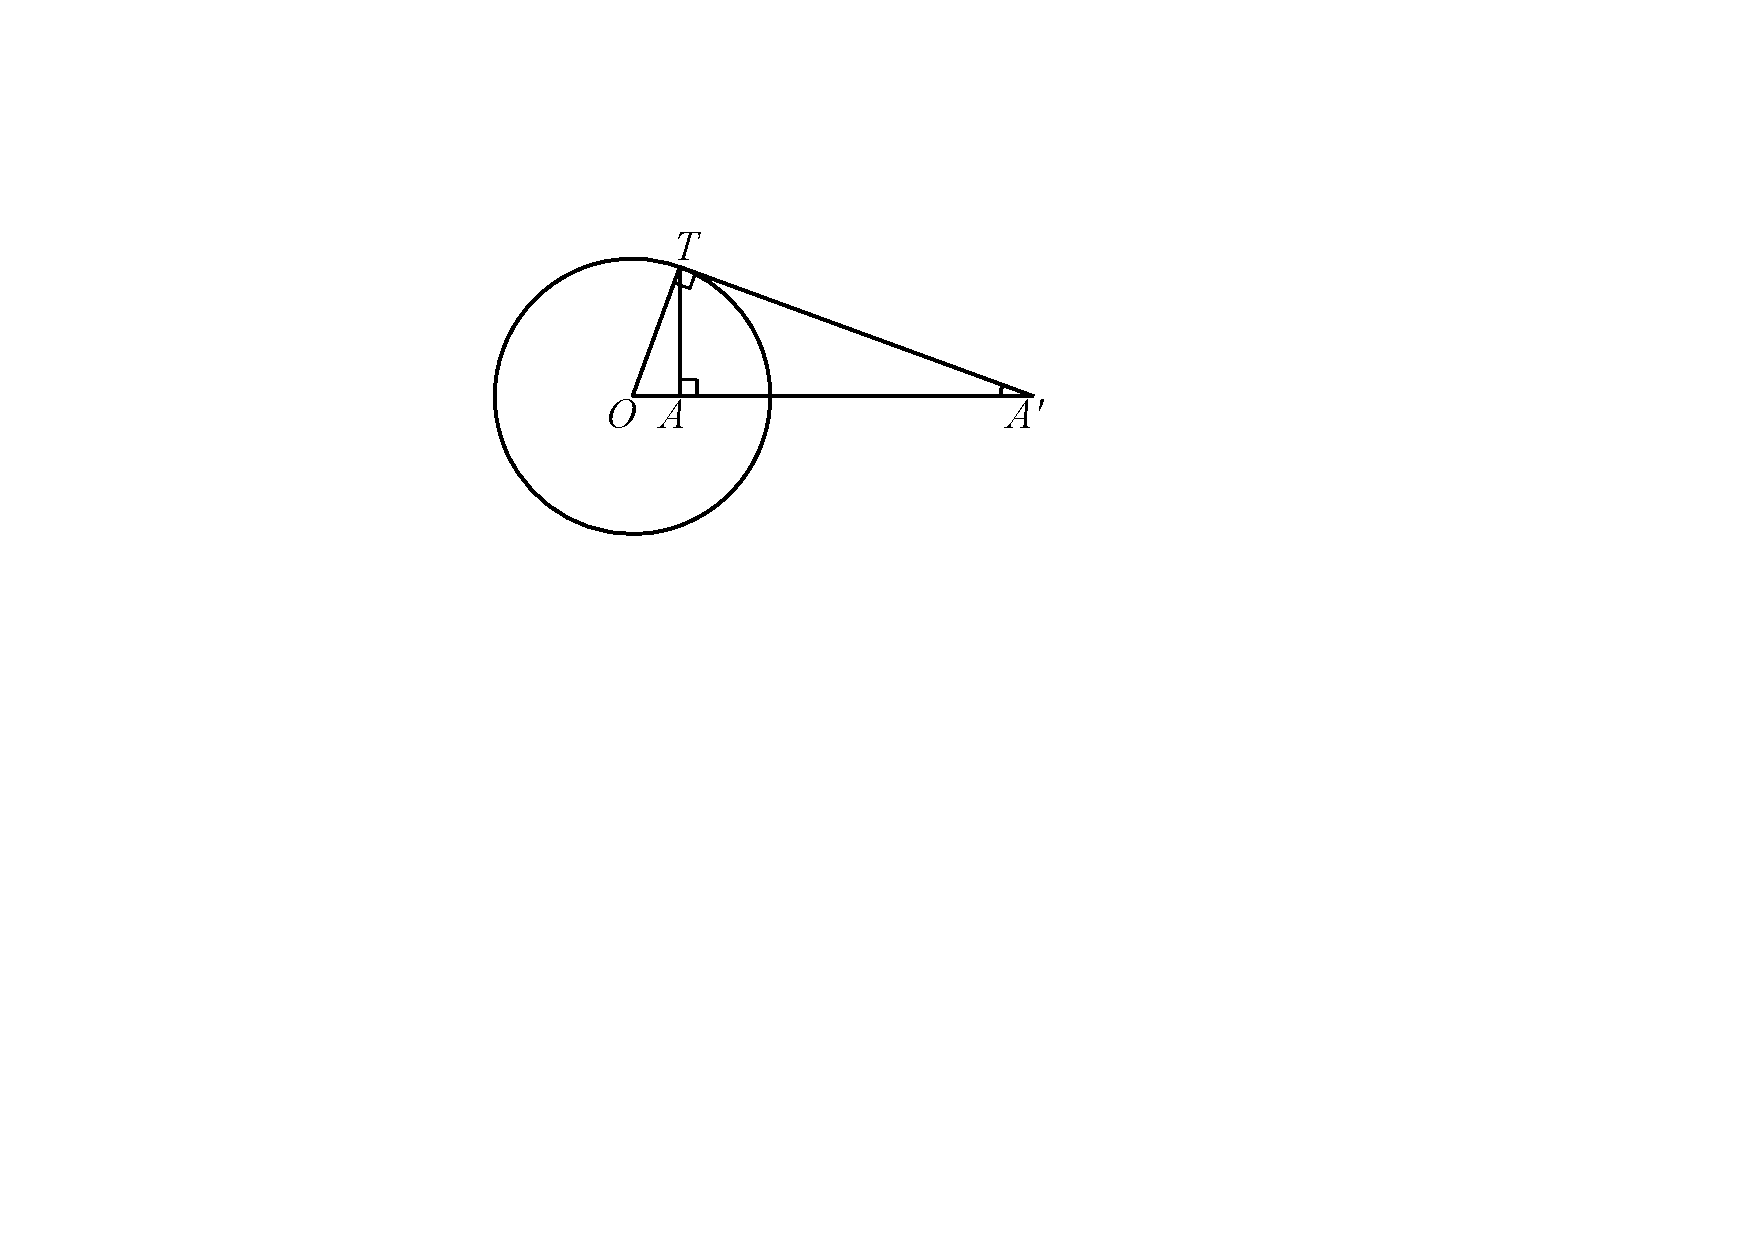
\includegraphics[width=0.5\linewidth]{圆的反演点}
\end{figure}

\item 椭圆上一点$ (x_0,y_0) $的切线斜率为\underline{\ \ifte 
    $ -\dfrac{b^2x_0}{a^2y_0} $\else \hspace{1cm} \fi\ },
切线方程为\underline{\ \ifte $ \dfrac{xx_0}{a^2}+\dfrac{yy_0}{b^2}=1 $
    \else \hspace{2cm} \fi\ }(换一半)。

\item 双曲线上一点$ (x_0,y_0) $的切线斜率为\underline{\ \ifte
    $ \dfrac{b^2x_0}{a^2y_0} $  \else \hspace{1cm} \fi\ },
切线方程为\underline{\ \ifte $ \dfrac{xx_0}{a^2}-
    \dfrac{yy_0}{b^2}=1 $\else \hspace{2cm} \fi\ }(换一半)。

\item 抛物线$ y^2=2px $上一点$ (x_0,y_0) $的切线斜率为
\underline{\ \ifte $ \dfrac{p}{y_0} $\else \hspace{1cm} \fi\ },
切线方程为\underline{\ \ifte $ yy_0=p(x+x_0) $
    \else \hspace{2cm} \fi\ }(换一半)。

\item 当点$ (x_0,y_0) $在椭圆外部时,直线$ \dfrac{xx_0}{a^2}+
\dfrac{yy_0}{b^2}=1 $表示椭圆的切点弦,即从点$ (x_0,y_0) $向椭圆
作两条切线,连接两个切点得到的弦。
\begin{figure}[H]
    \centering
    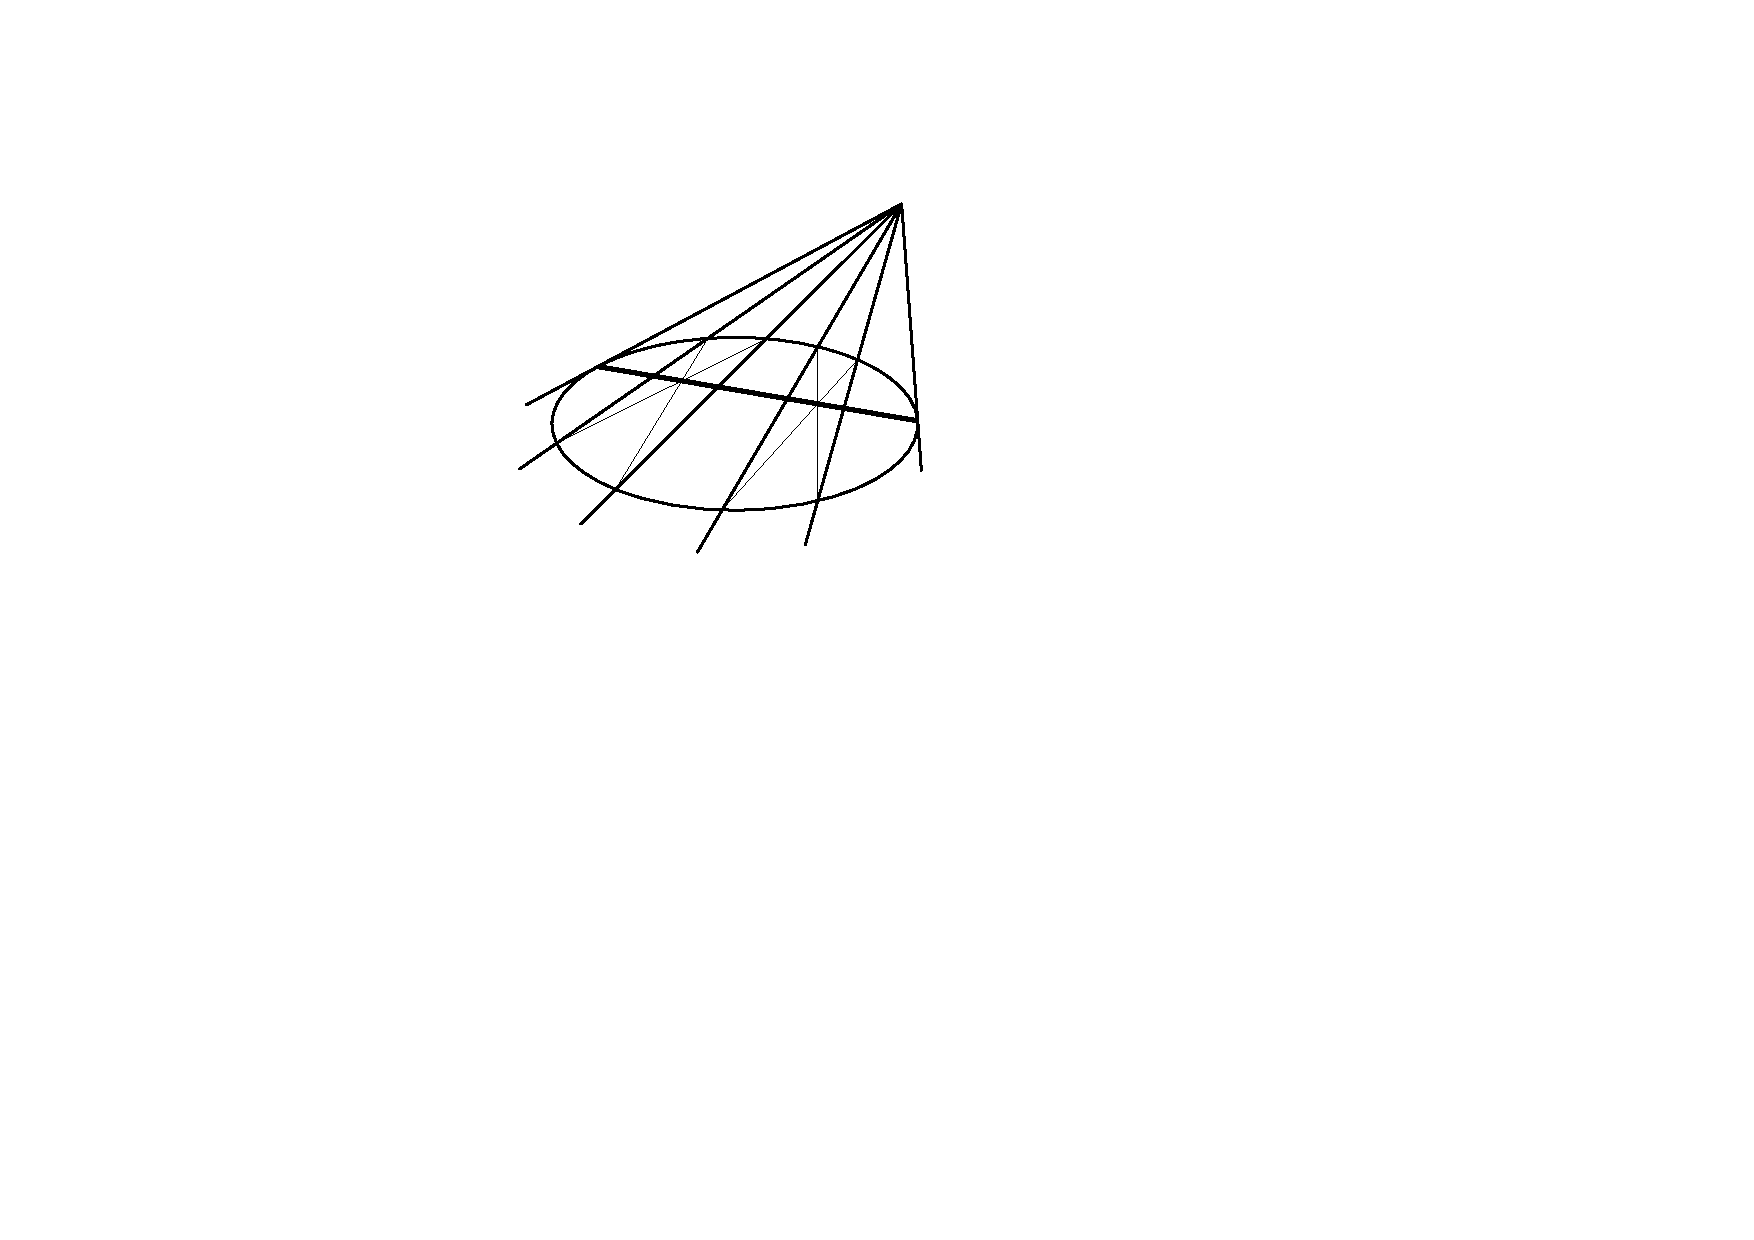
\includegraphics[width=0.4\linewidth]{椭圆-极点极线}
\end{figure}
从点$ (x_0,y_0) $出发作椭圆的两条割线,与椭圆有4个交点,
那么以这4个交点为顶点的四边形的对角线交点也在切点弦上。

\item 当点$ (x_0,y_0) $在椭圆内部时,直线$ \dfrac{xx_0}{a^2}+
\dfrac{yy_0}{b^2}=1 $与椭圆相离,从直线$ \dfrac{xx_0}{a^2}+
\dfrac{yy_0}{b^2}=1 $上的点向椭圆作两条切线,则切点弦过定点$ (x_0,y_0) $.
\begin{figure}[H]
    \centering
    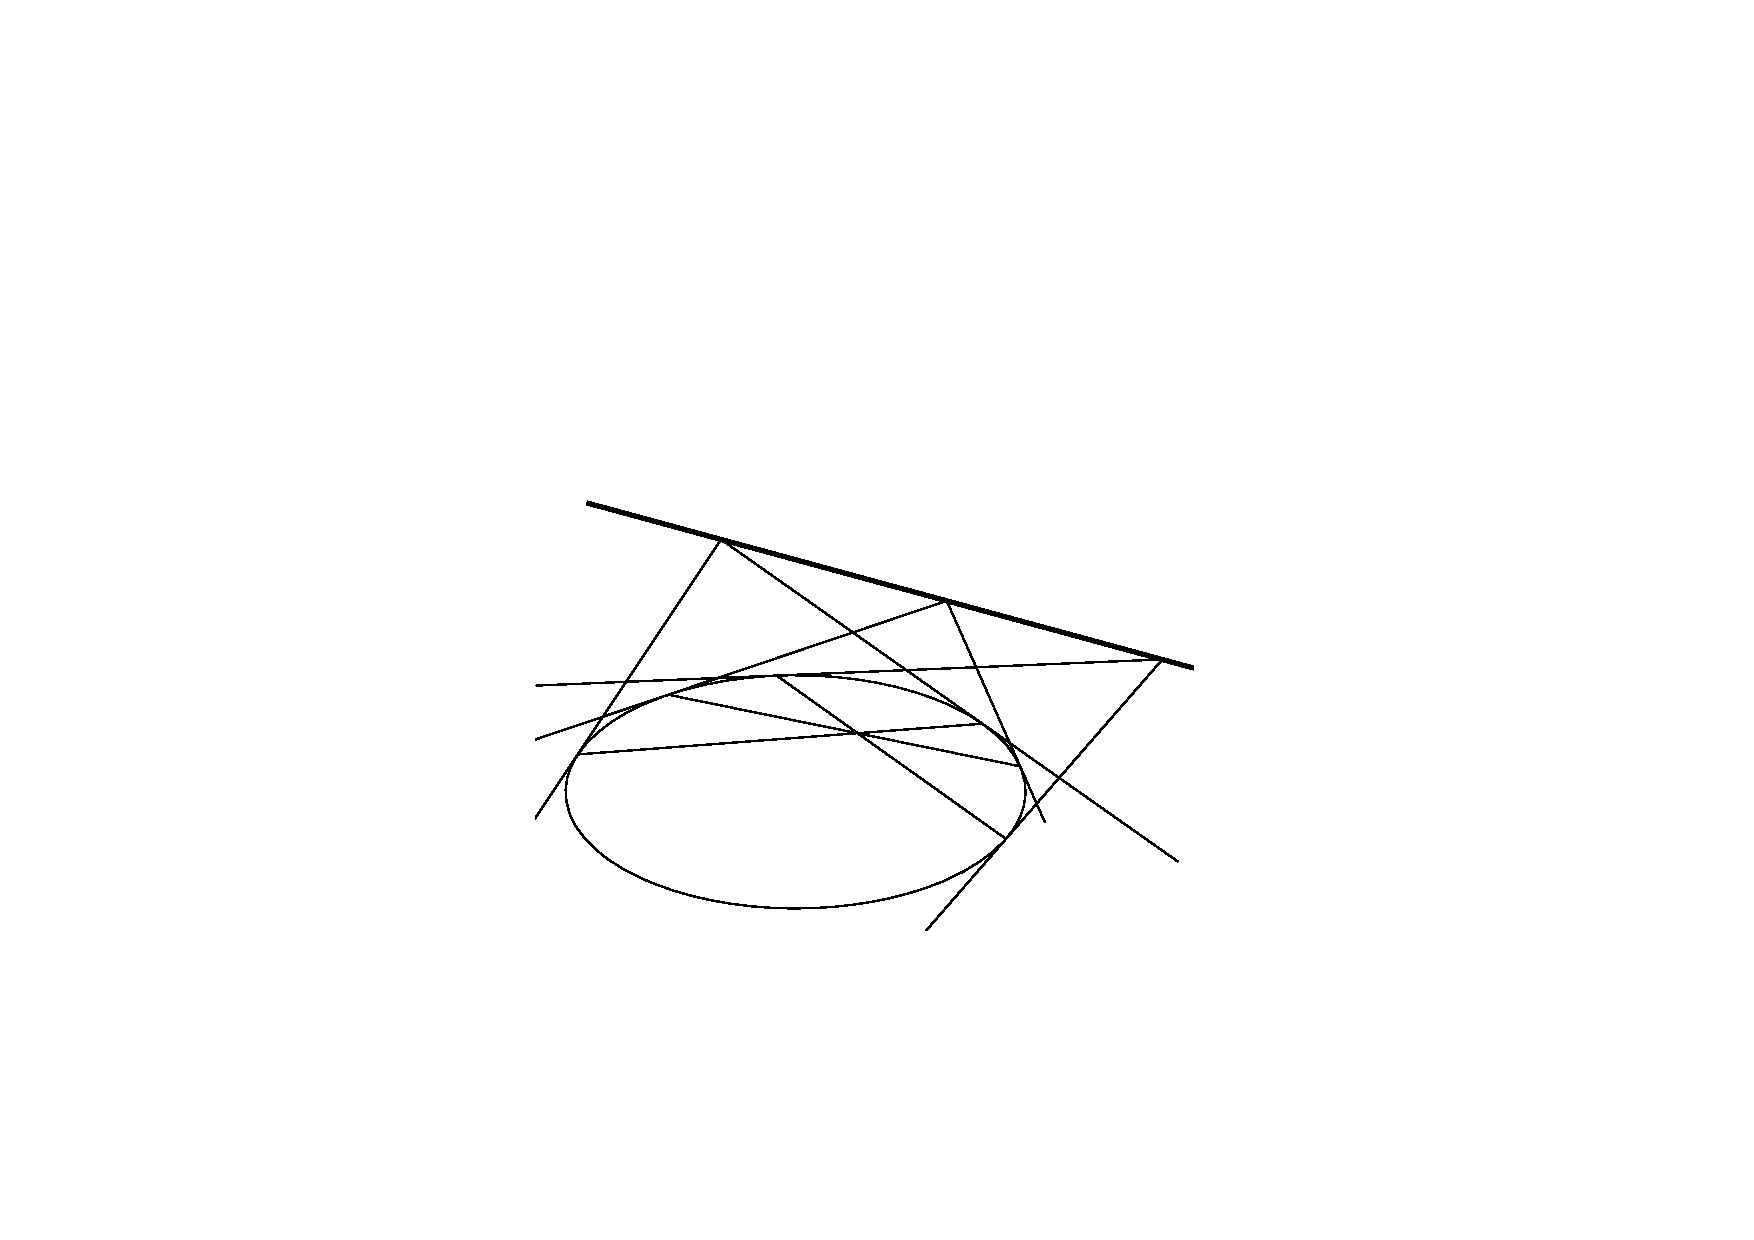
\includegraphics[width=0.5\linewidth]{配极原理-切点弦过定点}
\end{figure}

\item 椭圆上有不同的四点$ A,B,C,D $,假设$ AB $与$ CD $所在的直线交于
$ P $点,$ AD $与$ BC $所在的直线交于$ R $点,$ AC $与$ BD $交于$ Q $
点,则$ P $点的极线是$ QR $,$ Q $点的极线是$ PR $,
$ R $点的极线是$ PQ $,$ \Delta PQR $称为自极三角形。
\begin{figure}[H]
    \centering
    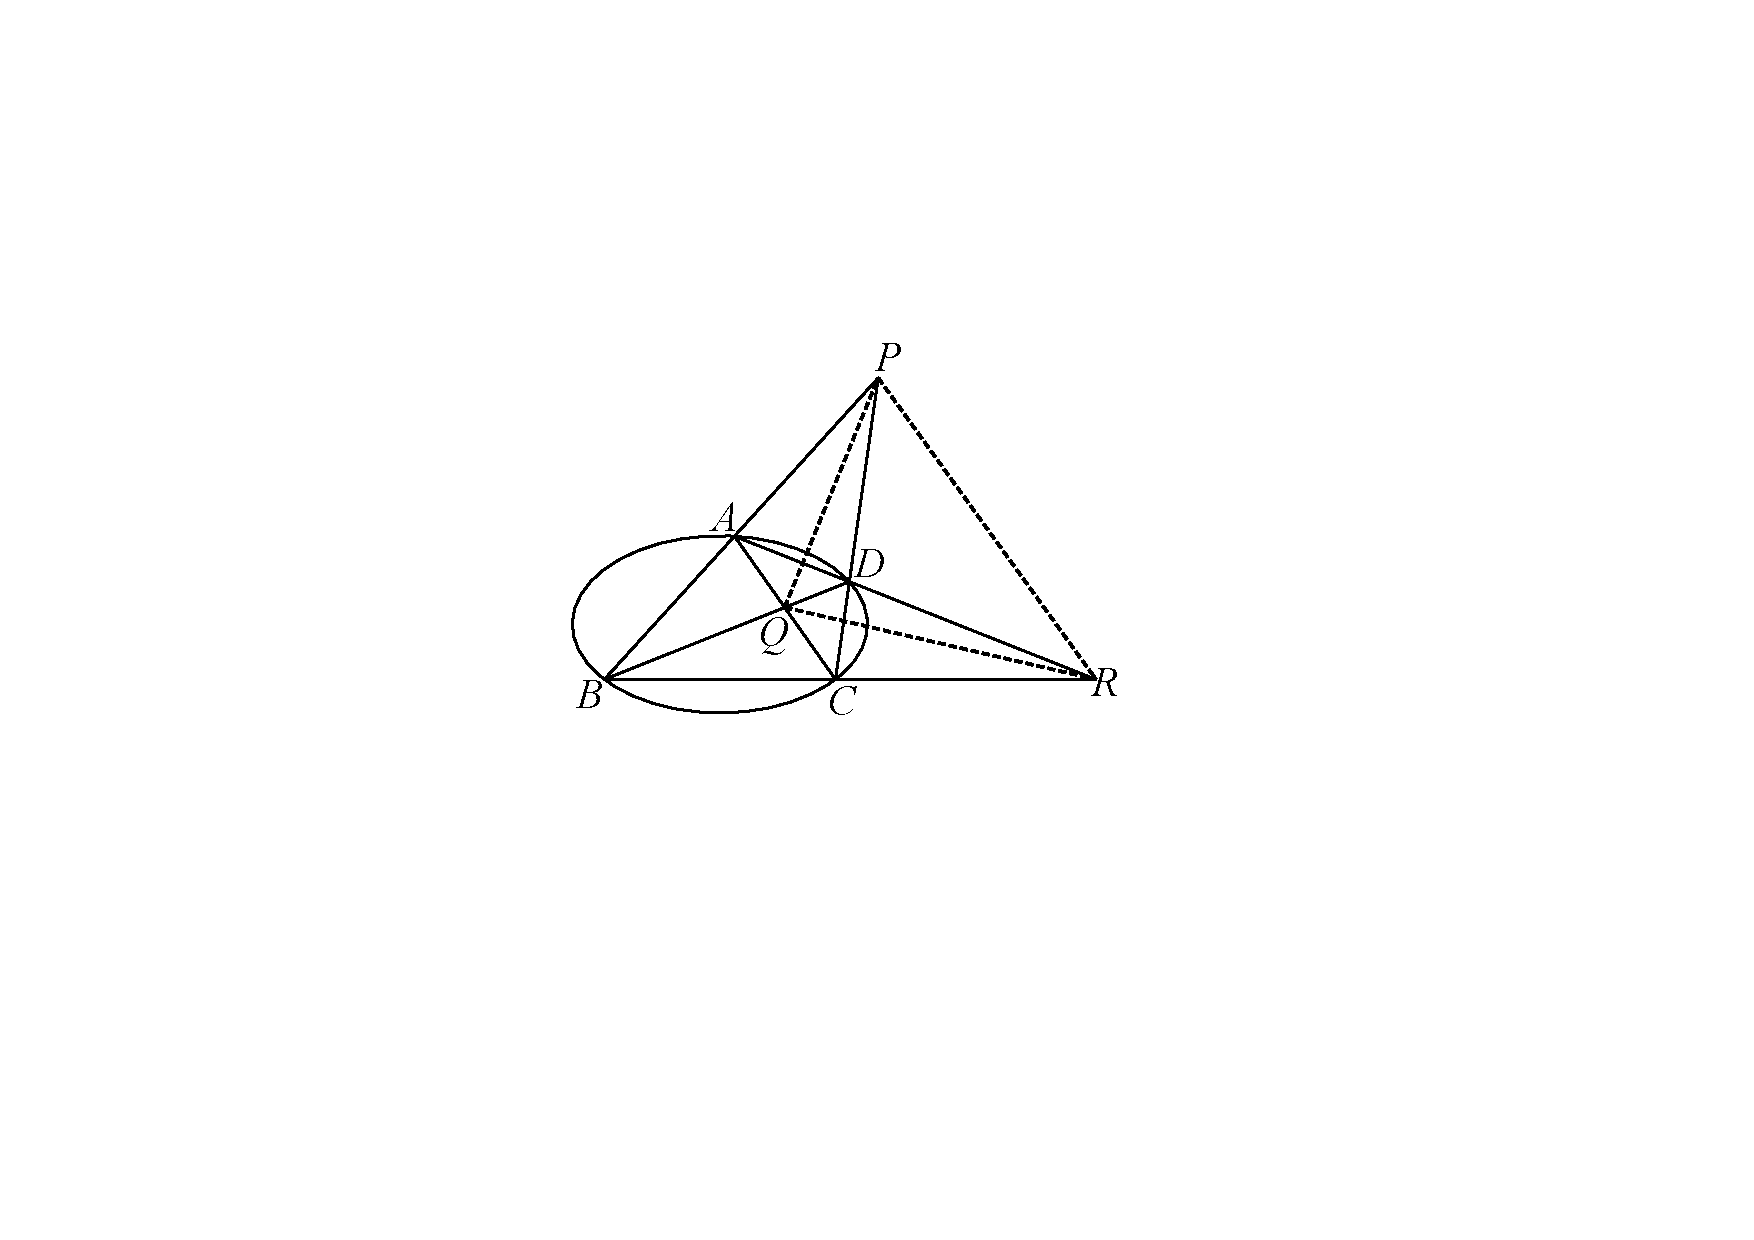
\includegraphics[width=0.6\linewidth]{自极三角形}
\end{figure}

\item 判断直线$ l:\ Ax+By+C=0 $与椭圆的位置关系,将直线方程变形为
\begin{gather*}
    \dfrac{\left(-\dfrac{Aa^2}{C}\right)x}{a^2}+
    \dfrac{\left(-\dfrac{Bb^2}{C}\right)y}{b^2}=1
\end{gather*}
设$ P\left(-\dfrac{Aa^2}{C},-\dfrac{Bb^2}{C}\right) $,
当$ P $点在椭圆内部时(即$ A^2a^2+B^2b^2<C^2 $),直线$ l $与椭圆相离;
当$ P $点在椭圆上时,直线$ l $与椭圆相切;
当$ P $点在椭圆外部时,直线$ l $与椭圆相交。

\item 椭圆$ \dfrac{x^2}{a^2}+\dfrac{y^2}{b^2}=1 (a>b>0) $的性质:
\begin{itemize}[leftmargin=-4pt]
\item 在椭圆外一点向椭圆做两条切线,切线夹角保持为$ \dfrac{\pi}{2} $时,
切线交点的轨迹方程为\underline{\ \ifte $ x_0^2+y_0^2=a^2+b^2 $
    \else \hspace{3cm} \fi\ }(蒙日圆,外准圆)

\item 从椭圆中心$ O $引出两条相互垂直的向径,
与椭圆分别交于$ P,Q $两点,从$ O $点向$ PQ $作垂线,
垂足为$ H $,那么$ H $点的轨迹也是一个圆(内准圆),圆的方程为
\underline{\ \ifte $ x^2+y^2=\dfrac{a^2b^2}{a^2+b^2} $
    \else \hspace{3cm} \fi\ }.
斜边长度$ |PQ| $的取值范围是:
\begin{gather*}
    \underline{\ \ifte \dfrac{2ab}{\sqrt{a^2+b^2}} \else \hspace{2cm} \fi\ }
    \leq |PQ| \leq 
    \underline{\ \ifte \sqrt{a^2+b^2} \else \hspace{2cm} \fi\ }
\end{gather*}
$ \Delta OPQ $的面积的取值范围是:
\begin{gather*}
    \underline{\ \ifte \dfrac{a^2b^2}{a^2+b^2}\else \hspace{2cm} \fi\ }
    \leq S_{\Delta OPQ} \leq 
    \underline{\ \ifte \dfrac{1}{2}ab \else \hspace{2cm} \fi\ }
\end{gather*}

\item 以下三种情形,斜率之积为定值。
\begin{figure}[H]
    \centering
    \includegraphics[width=0.95\linewidth]{"椭圆-两直线斜率之积-删除圆"}
\end{figure}
$ k_{AP}\cdot k_{BP}=k_{OT}\cdot k_{PT}=k_{OM}\cdot k_{AB}=
\underline{\ \ifte -\dfrac{b^2}{a^2}\else \hspace{2cm} \fi\ } $.

\item $AB,CD$是椭圆的两条相交弦,交点为$P$,且$ AB,\ CD $
的斜率互为相反数,则$ |PA|\cdot|PB|=\underline{\ \ifte 
    |PC|\cdot|PD| \else \hspace{2cm} \fi\ } $. 

\item $^*$ 椭圆上任意一点$ P(x_0,y_0) $,过$ P $点作两条相互垂直的直线,
这两条直线与椭圆的除$ P $点之外的交点分别是$ Q,R $,那么线段$ QR $过定点
\begin{gather*}
    \left(\dfrac{(a^2-b^2)x_0}{a^2+b^2},-\dfrac{(a^2-b^2)y_0}{a^2+b^2}\right)
\end{gather*}

\item $^*$ 过椭圆内部一点$ M(x_0,y_0) $作椭圆的两条垂直弦$ PQ,RS $,
弦$ PQ,RS $的中点分别为$ K,L $,那么线段$ KL $过定点
\begin{gather*}
    \left(\dfrac{a^2x_0}{a^2+b^2},\dfrac{b^2y_0}{a^2+b^2}\right)
\end{gather*}

\item 椭圆上任意一点$ P(x_0,y_0) $,过$ P $点作两条斜率互为
相反数的直线,这两条直线与椭圆的除$ P $点之外的交点分别是$ Q,R $,
那么直线$ QR $的斜率是定值,且与过$ P $的切线的斜率互为
\underline{\ \ifte 相反数\else \hspace{2cm} \fi\ }。

\item 在椭圆的长轴$ AB $上有一定点$ M(m,0) $,过点$ M $作椭圆的弦$ CD $,
记直线$ AC,BD $的斜率分别为$ k_{1},k_{2} $,则 \\
\ding{172} $ \dfrac{k_{1}}{k_{2}} $是定值;\\
\ding{173}  $ AC,BD $延长线的交点的轨迹方程是
\underline{\ \ifte $ x=\dfrac{a^2}{m} $
    \else \hspace{1.5cm} \fi\ },即点$ M $关于椭圆的极线;\\
\ding{174} 设\ding{173}中的极线与$ AB $延长线的交点为$ H $,
    则$ CH, DH $的斜率互为\underline{\ \ifte 相反数
        \else \hspace{2cm} \fi\ }。

\item $P$为椭圆上一点,$F_1,F_2$是椭圆的左右焦点,$\angle F_1PF_2=\theta $,
则 $ S_{\Delta F_1PF_2}=\underline{\ \ifte b^{2}\tan\dfrac{\theta}{2}
    \else \hspace{1cm} \fi\ } $. 
   
\item $ F_1,F_2 $是椭圆的两个焦点,椭圆上一点$ P $处的切线$ PT $平分$ \Delta
PF_1F_2 $在点$ P $处的外角。焦点在直线$ PT $上的投影点的轨迹是以长轴为直径的圆。
以$ PF_1 $(或$ PF_2 $)为直径的圆必与以长轴为直径的圆
\underline{\ \ifte 内切\else \hspace{1cm} \fi\ }。

\item 设椭圆的左右两个顶点为$ A_1(-a,0),A_2(a,0) $,与$ y $轴平行的直线交椭圆于
$ P_1,P_2 $时,$ A_1P_1 $与$ A_2P_2 $的交点的轨迹方程是
\underline{\ \ifte $ \dfrac{x^2}{a^2}-\dfrac{y^2}{b^2}=1 $
    \else \hspace{2cm} \fi\ }.    

\end{itemize}

\item 双曲线$ \dfrac{x^2}{a^2}-\dfrac{y^2}{b^2}=1 $的性质:
\begin{itemize}[leftmargin=-4pt]
\item 从不在双曲线上的一点做双曲线的两条切线,如果两条切线垂直,那么切线交点的轨迹
也是一个圆(蒙日圆,外准圆),圆的方程为\underline{\ \ifte 
    $ x^2+y^2=|a^2-b^2| $ \else \hspace{2cm} \fi\ }.

\item 从双曲线的中心$ O $引出两条相互垂直的向径,
与双曲线分别交于$ P,Q $两点,从$ O $
点向$ P,Q $作垂线,垂足为$ H $,那么$ H $点的轨迹也是一个圆(内准圆),
内准圆的方程是\underline{\ \ifte $ x^2+y^2=\dfrac{a^2b^2}{b^2-a^2} $
    \else \hspace{2cm} \fi\ }.
双曲线内准圆存在的充要条件是虚轴大于实轴,即离心率大于$ \sqrt{2} $.

\item $^*$ 双曲线上任意一点$ P(x_0,y_0) $,过$ P $点作两条相互垂直的直线,这两条直线
与双曲线的除$ P $点之外的交点分别是$ Q,R $,那么线段$ QR $过定点。
\begin{gather*}
    \left(\dfrac{(a^2+b^2)x_0}{a^2-b^2},-\dfrac{(a^2+b^2)y_0}{a^2-b^2}\right)
\end{gather*}
必须满足$ a\neq b $,定点才存在。

\item $^*$ 过平面上任意一点$ M(x_0,y_0) $作双曲线的两条垂直弦$ PQ,RS $,
弦$ PQ,RS $的中点分别为$ K,L $,那么线段$ KL $过定点。
\begin{gather*}
    \left(\dfrac{a^2x_0}{a^2-b^2},-\dfrac{b^2y_0}{a^2-b^2}\right)
\end{gather*}
必须满足$ a\neq b $,定点才存在。

\item 双曲线上任意一点$ P(x_0,y_0) $,过$ P $点作两条斜率互为
相反数的直线,这两条直线与双曲线的除$ P $点之外的交点分别是$ Q,R $,
那么直线$ QR $的斜率是定值,且与过$ P $的切线的斜率互为
\underline{\ \ifte 相反数\else \hspace{2cm} \fi\ }。

\item $P$为双曲线上一点,$F_1,F_2$是双曲线的左右焦点,$\angle F_1PF_2=\theta $,
则$ S_{\Delta F_1PF_2}=\underline{\ \ifte \dfrac{b^2}{\tan\frac{\theta}{2}} 
    \else \hspace{1cm} \fi\ } $.

\item 设$ k>0 $,则等轴双曲线$ y=\dfrac{k}{x} $的实半轴和虚半轴的长度均为
\underline{\ \ifte $ \sqrt{2k} $\else \hspace{1cm} \fi\ },
焦点坐标是\underline{\ \ifte $ (\pm\sqrt{2k},\pm\sqrt{2k}) $
    \else \hspace{2cm} \fi\ }.


\end{itemize}

\item 抛物线$ y^2=2px $的性质:
\begin{itemize}[leftmargin=-4pt]
    
\item 抛物线的焦点为$ F $,顶点为$ O $,过焦点的直线与抛物线交于$ P(x_1,y_1),
Q(x_2,y_2) $两点,则 \\ $ \dfrac{1}{|FP|}+\dfrac{1}{|FQ|}=
\dfrac{1-\cos\theta}{p}+\dfrac{1-\cos\theta}{p}=
\underline{\ \ifte \dfrac{2}{p}\else \hspace{2cm} \fi\ } $;\\
$ |FP|+|FQ|=\dfrac{p}{1-\cos\theta}+\dfrac{p}{1+\cos\theta}
=\underline{\ \ifte \dfrac{2p}{\sin^2\theta}\else \hspace{2cm} \fi\ } $;\\
$ y_1y_2=\underline{\ \ifte -p^2 \else \hspace{2cm} \fi\ },\ 
x_1x_2=\dfrac{y_1^2}{2p}\cdot \dfrac{y_2^2}{2p}=
\underline{\ \ifte \dfrac{p^2}{4}\else \hspace{2cm} \fi\ } $;\\
$ S_{\Delta OPQ}=\dfrac{1}{2}\cdot \dfrac{p}{2}\cdot\Big(\dfrac{2p}{\sin^2\theta}\cdot \sin\theta\Big)=
\underline{\ \ifte \dfrac{p^2}{2\sin\theta}\else \hspace{2cm} \fi\ } $.

\item 抛物线的对称轴上有一个固定点$ M(x_0,0) $,过$ M $的直线与
抛物线交于$ P(x_1,y_1),Q(x_2,y_2) $两点,则\\ $ y_1y_2=
\underline{\ \ifte -2px_0\else \hspace{2cm} \fi\ } $,
$ x_1x_2=\dfrac{y_1^2}{2p}\cdot \dfrac{y_2^2}{2p}=
\underline{\ \ifte x_0^2\else \hspace{2cm} \fi\ } $.

\item 抛物线的顶点为$ O $,$ A,B $两点在抛物线上,
若$ \vec{OA}\cdot\vec{OB}=-p^2 $,则直线$ AB $过定点
\underline{\ \ifte $ (p,0) $\else \hspace{2cm} \fi\ }.

\item 从准线上的一点$ P\Big(-\dfrac{p}{2},y_0\Big) $向抛物线作两条切线,
设切点分别为$ Q,R $,则这两条切线$ PQ,PR $相互\underline{\ 
    \ifte 垂直\else \hspace{2cm} \fi\ }。设抛物线焦点为$ F $,
那么$ QR $恒过\underline{\ \ifte 焦点 \else \hspace{2cm} \fi\ },
且$ PF\perp \underline{\ \ifte QR\else \hspace{2cm} \fi\ } $.

\item 抛物线上任意一点$ P(x_0,y_0) $,过$ P $点作两条相互垂直的直线,
这两条直线与抛物线的除$ P $点之外的交点分别是$ Q,R $,那么线段$ QR $过定点
\underline{\ \ifte $ (x_0+2p,-y_0) $\else \hspace{2cm} \fi\ }.

\item 抛物线上任意一点$ P(x_0,y_0) $,过$ P $点作两条斜率互为
相反数的直线,这两条直线与抛物线的除$ P $点之外的交点分别是$ Q,R $,
那么直线$ QR $的斜率是定值,且与过$ P $的切线的斜率互为
\underline{\ \ifte 相反数\else \hspace{2cm} \fi\ }。

%\item 

\end{itemize}

\item $^*$ 彭赛列(Poncelet)闭合定理:给定两条圆锥曲线$ \Gamma_1 $和$ \Gamma_2 $,
若存在一个$ n\ (n\geq 3) $边形满足:内接于$ \Gamma_1 $且外切于$ \Gamma_2 $,
则必然存在无数个这样的$ n $边形满足该性质(同时内接和外切)。

\item $^*$ 三角形的内心和外心的距离为$ \sqrt{R(R-2r)} $,
其中$ R $为外接圆半径,$ r $为内切圆半径。
假设一个半径为$ r $的小圆位于一个半径为$ R $大圆的内部(两个圆没有交点),
若$ 2r<R $且两个圆的圆心距恰好等于$ \sqrt{R(R-2r)} $,那么存在无穷多个三角形,
分别以这两个圆为内切圆和外接圆。

\item $^*$ 蝴蝶定理:在圆锥曲线中,过弦$ PQ $的中点$ M $任作两条弦$ AB,CD $,
直线$ AC,BD $交$ PQ $于点$ E,F $,则$ ME=EF $.
\begin{figure}[H]
    \centering
    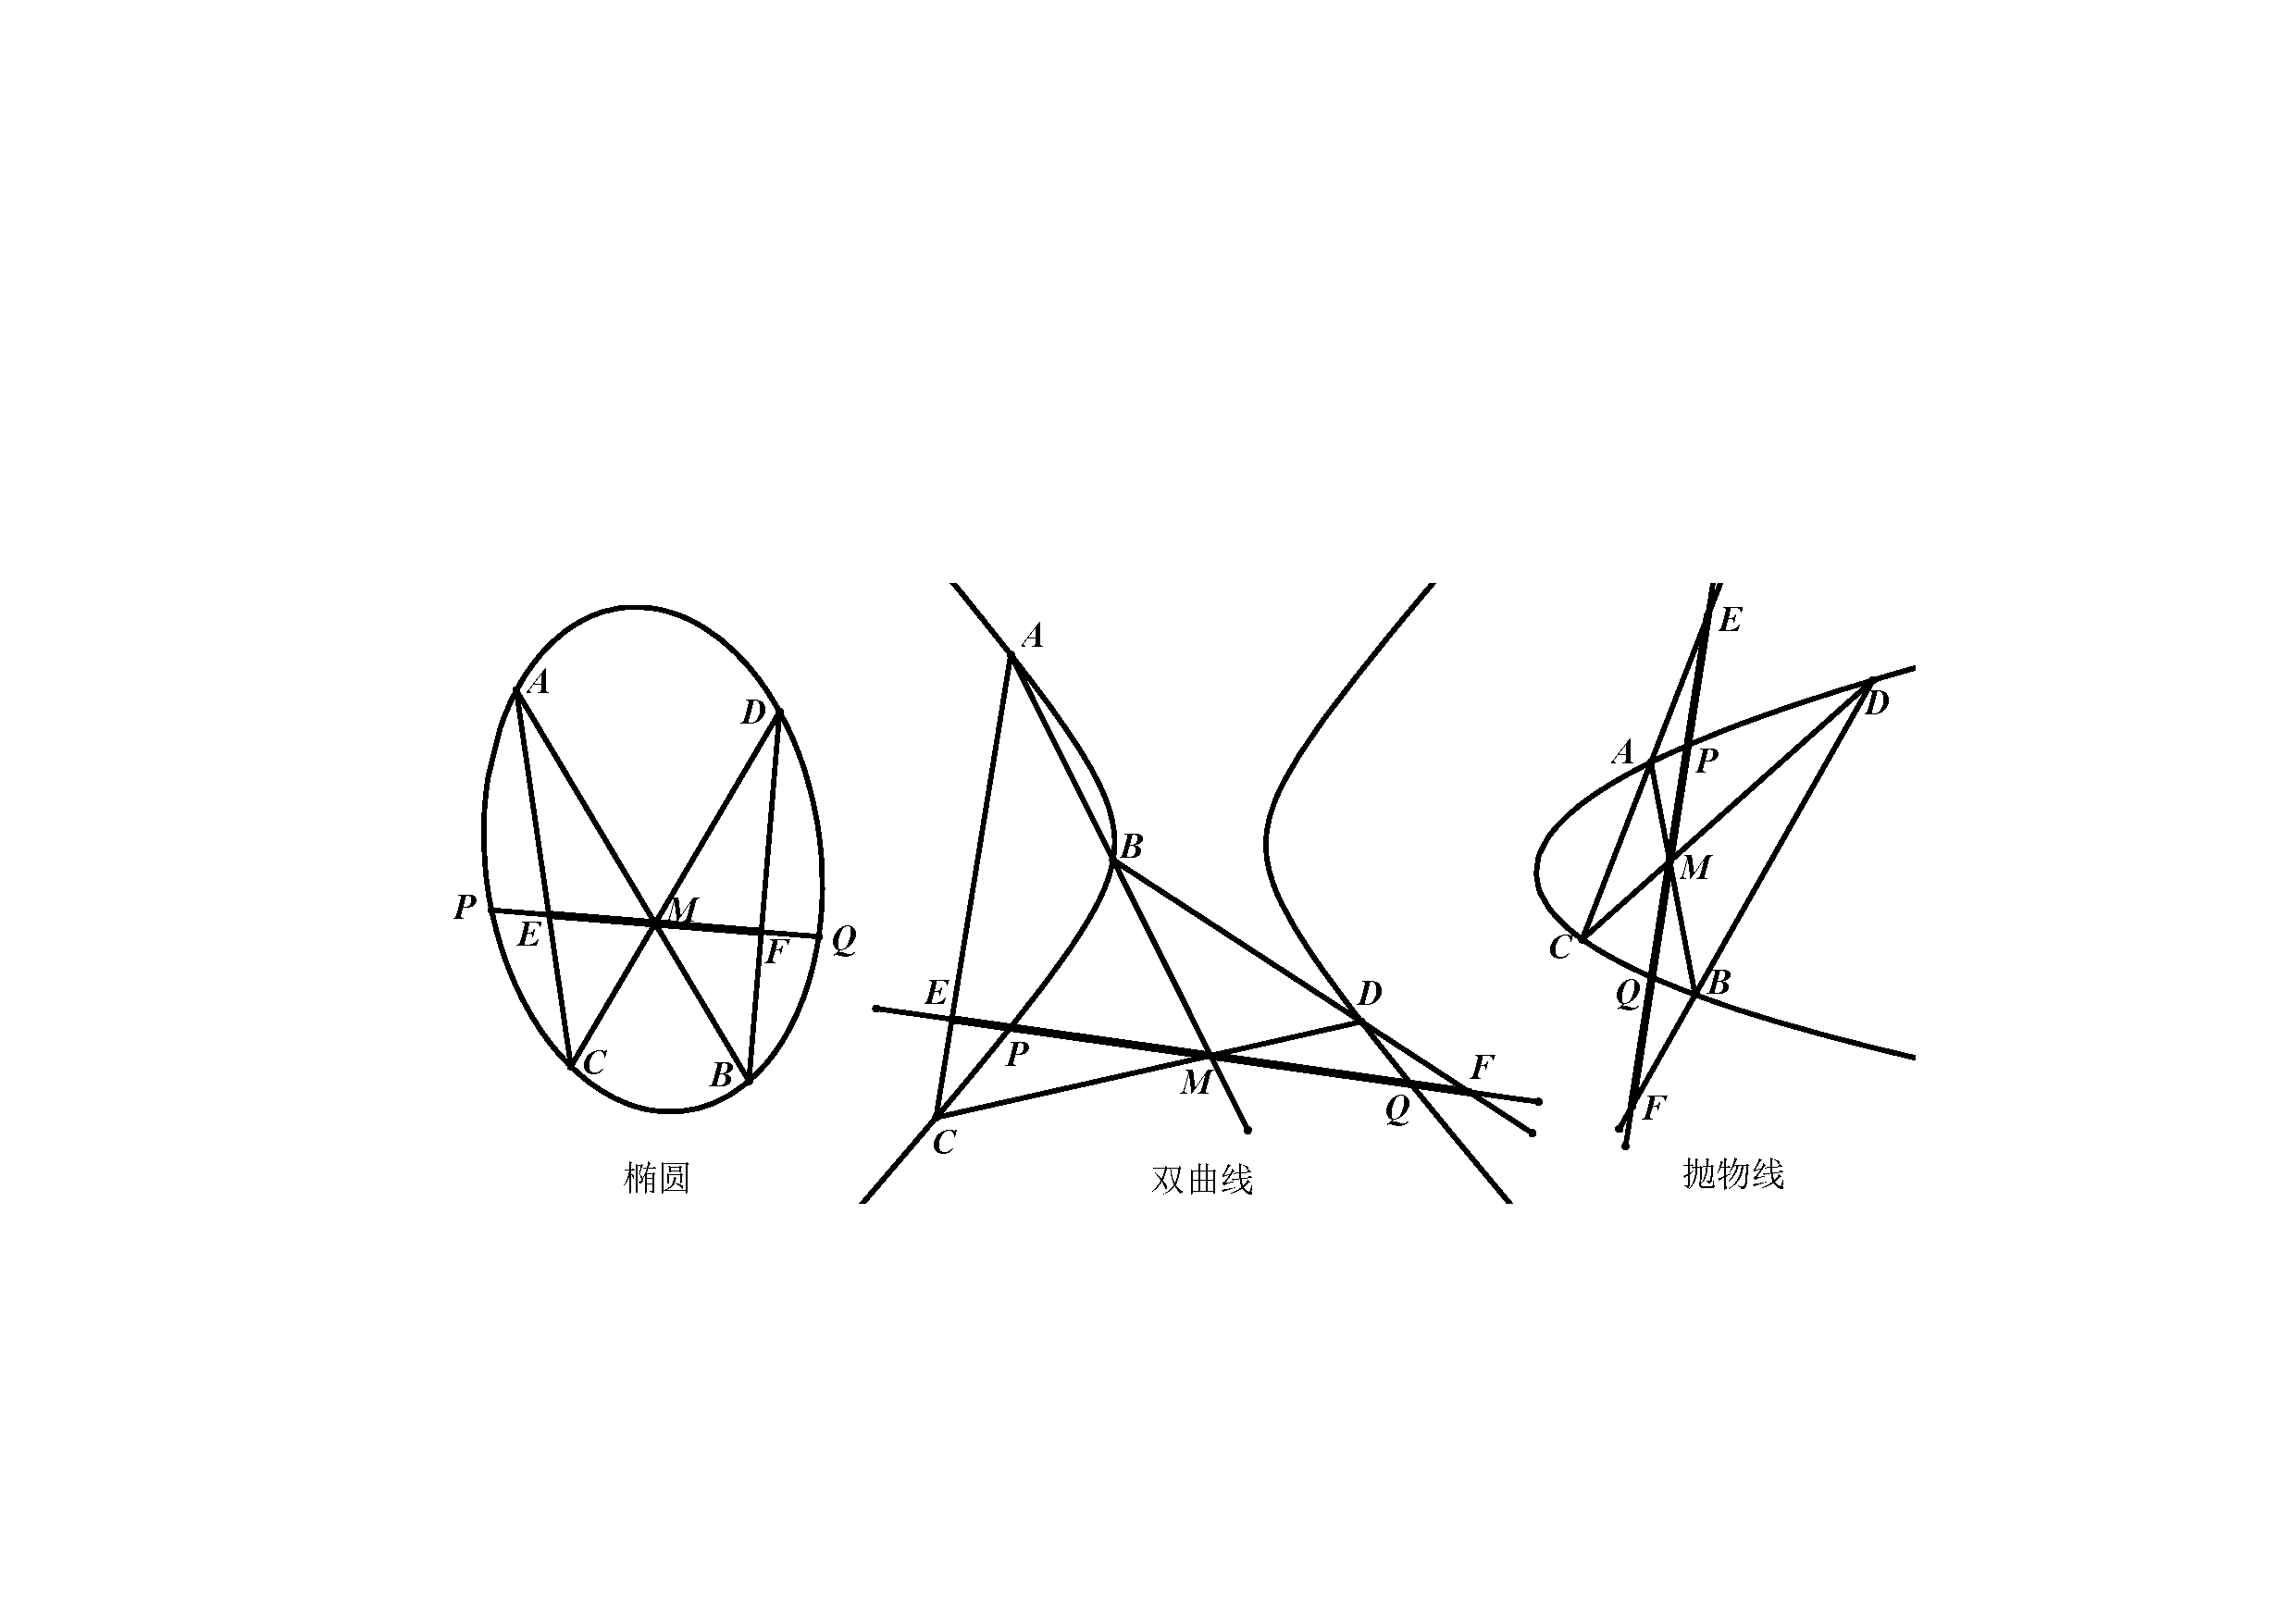
\includegraphics[width=0.95\linewidth]{蝴蝶定理}
\end{figure}


\subsection{零散考点}

\item 集合的3个特征:\underline{\ \ifte 
 确定性、互异性、无序性 \else \hspace{3.5cm} \fi\ } 。

\item $ \pi\approx 3.141592653 $的分数近似值:\\ $ \dfrac{22}{7} 
\approx 3.142857,\ \dfrac{355}{113}\approx 3.14159292 $. 

\item 三次方程韦达定理:$ (a\neq 0) $,
\begin{align*}
    &\ x^3+\dfrac{b}{a}x^2+\dfrac{c}{a}x+\dfrac{d}{a} \\
   =&\ (x-x_1)(x-x_2)(x-x_3)=0
\end{align*}
$ x_1+x_2+x_3= $\underline{\ \ifte $ -\dfrac{b}{a} $\else 
    \hspace{2cm} \fi\ };\\
$ x_1x_2+x_1x_3+x_2x_3= $\underline{\ \ifte $ \dfrac{c}{a} $ 
    \else \hspace{2cm} \fi\ };\\
$ x_1x_2x_3= $\underline{\ \ifte $ -\dfrac{d}{a} $ \else \hspace{2cm} \fi\ }.

\item 因式分解:
\begin{align*}
    a^3\pm b^3 &=\underline{\ \ifte (a\pm b)(a^2\mp ab+b^2)
        \else \hspace{4cm} \fi\ } \\
    a^4-b^4 &=\underline{\ \ifte (a-b)(a^3+a^2b+ab^2+b^3)
        \else \hspace{4cm} \fi\ } \\
          &=(a-b)(a+b)(a^2+b^2) \\
    a^n-b^n &=(a-b)(\underline{\ \ifte 
        a^{n-1}+a^{n-2}b+\cdots+b^{n-1}
        \else \hspace{4cm} \fi\ })
\end{align*}
\begin{align*}
   & a^3+b^3+c^3-3abc=\\ & \underline{\ \ifte 
    (a+b+c)(a^2+b^2+c^2-ab-bc-ca) \else \hspace{6cm} \fi\ } 
\end{align*}

\item 锥体(圆锥、棱锥)体积公式:$ V=\underline{\ \ifte 
    \dfrac{1}{3}Sh\else \hspace{1cm} \fi\ } $,\\
$ S $为底面积,$ h $为锥体高度。

\item 圆台或棱台的体积:$ V=\underline{\ \ifte 
\dfrac{1}{3}(S+\sqrt{SS'}+S')h\else \hspace{3cm} \fi\ } $,\\
$ S,S' $为两个底面积,$ h $为台体高度(两个底面间的距离)。


}
\end{enumerate}
\end{multicols}   






